%% LyX 2.3.7 created this file.  For more info, see http://www.lyx.org/.
%% Do not edit unless you really know what you are doing.
\documentclass[english]{article}
\usepackage[T1]{fontenc}
\usepackage[latin9]{inputenc}
\usepackage{float}
\usepackage{textcomp}
\usepackage{enumitem}
\usepackage{amsmath}
\usepackage{amsthm}
\usepackage{amssymb}
\usepackage{stackrel}
\usepackage{graphicx}

\makeatletter
%%%%%%%%%%%%%%%%%%%%%%%%%%%%%% Textclass specific LaTeX commands.
\numberwithin{equation}{section}
\numberwithin{figure}{section}
\newlength{\lyxlabelwidth}      % auxiliary length 

%%%%%%%%%%%%%%%%%%%%%%%%%%%%%% User specified LaTeX commands.
%=====================================================================
% Identification
%=====================================================================
\NeedsTeXFormat{LaTeX2e}

\RequirePackage{fancyhdr}
\RequirePackage[top=1in,bottom=1in,left=1in,right=1in]{geometry}
\RequirePackage{graphicx}
\RequirePackage{empheq}
\RequirePackage{ifthen}


%\RequirePackage{jhwgraphics} Another personal style file I use.


%=====================================================================
% Commands
%=====================================================================

  \setlength{\headheight}{15pt}
  \lhead{\@author}\chead{\@title}\rhead{Distributions}
%{\today}
  \lfoot{}\cfoot{\thepage}\rfoot{}
  \pagestyle{fancy}

  }
                                          %PDFLaTeX
  \RequirePackage[pdftex,bookmarks=true]{hyperref}
  \hypersetup{ %
    pdfauthor   = {\@author},
    pdftitle    = {\@title},
    pdfcreator  = {LaTeX with hyperref package},
    pdfproducer = {dvips + ps2pdf}
  }
\pdfadjustspacing=1

\makeatother

\usepackage{babel}
\begin{document}

\section{Discrete Distributions}

\subsection{Bernoulli and Binomial}

The Bernoulli distribution is the simplest case of the Binomial distribution,
where we only have one trial $(n=1).$ Let us say that $X$ is distributed
$\text{Bern}(p)$. We know the following: A trial is performed with
probability $p$ of \textquotedblleft success\textquotedblright ,
and $X$ is the indicator of success: 1 means success, 0 means failure.

Let us say that $X$ is distributed $\text{Bin}(n,p)$. We know the
following: X is the number of \textquotedblleft successes\textquotedblright{}
that we will achieve in $n$ independent trials, where each trial
is either a success or a failure, each with the same probability $p$
of success. We can also write $X$ as a sum of multiple independent
$\text{Bern}(p)$ random variables. Let $X\sim\text{Bin}(n,p)$ and
$X_{j}\sim\text{Bern}(p)$, where all of the Bernoullis are independent.
Then $X=X_{1}+X_{2}+\ldots+X_{n}$.
\begin{enumerate}
\item PMF, MGF, mean and variance of $X\sim\text{Binom}(n,p)$
\begin{enumerate}
\item \textbf{PMF}: 
\[
f(x)={n \choose x}p^{x}(1-p)^{n-x},
\]

\begin{center}
$x=0,1,...n$
\par\end{center}

\begin{center}
$0<p<1$
\par\end{center}
\item \textbf{MGF}: $M_{X}(t)=[(1-p)+pe^{t}]^{n}$
\item \textbf{Mean and Variance}: 
\[
E[X]=np,\,\,Var(X)=np(1-p)
\]
\end{enumerate}
\begin{figure}[H]
\begin{centering}
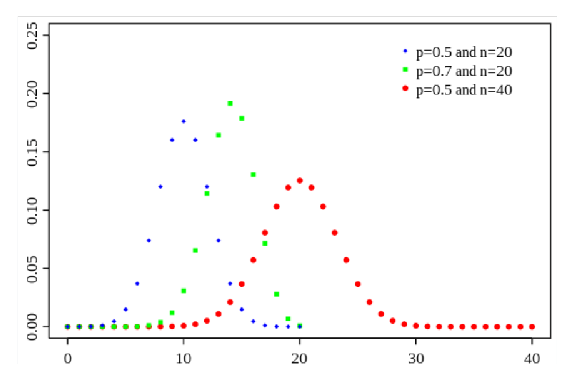
\includegraphics[width=0.25\paperwidth]{images/dist_binomial} 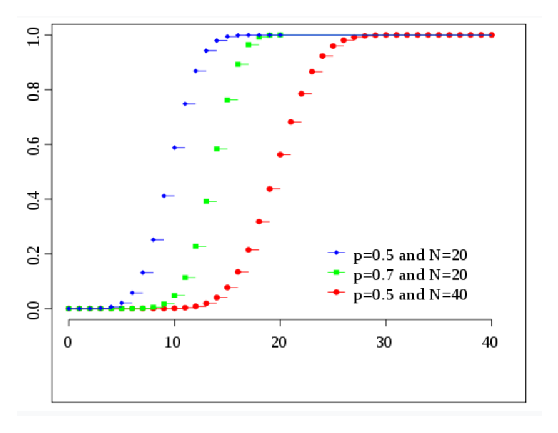
\includegraphics[width=0.25\paperwidth]{images/cdf_binomial}
\par\end{centering}
\caption{Bernoulli PMF (left) CDF (right)}
\end{figure}

\item \textbf{Additive property}

If for $i=1,2,...,k$, $X_{i}\sim\text{Binom}(n_{i},p)$, then $\sum_{i=1}^{k}X_{i}\sim\text{Binom}(\sum_{i=1}^{k}n_{i},p)$
\end{enumerate}
\begin{enumerate}[resume]
\item Random sample $X_{1},...,X_{n}\sim\text{Ber}(p)$ where $p$ is \textbf{target
parameter}: exponential family? sufficient statistic? minimal sufficient
statistic? complete statistic? Fisher information? UMVUE?
\begin{enumerate}
\item \textbf{Exponential family} form: $(1-p)^{n}\exp\left(\mathop{\sum_{i=1}^{n}x_{i}log\frac{p}{1-p}}\right)$
\item \textbf{Minimal sufficient and complete statistic}: $\sum_{i=1}^{n}X_{i}$
\item \textbf{Fisher information}: $\frac{n}{p(1-p)}$
\item \textbf{UMVUE}: $\frac{1}{n}\sum_{i=1}^{n}X_{i}$
\item \textbf{MLE} $\hat{p}=\frac{1}{n}\sum_{i=1}^{n}X_{i}$
\end{enumerate}
\item \textbf{Conjugate prior} of $p$?

$X|p\sim\text{Binom}(n,p)$

$p\sim\text{beta}(\alpha,\beta)$.

\textbf{Posterior} distribution $p|(X=x)\sim\text{beta}(\alpha+\mathop{\sum_{i=1}^{n}x_{i}},n+\beta-\sum_{i=1}^{n}x_{i})$
\item \textbf{Related Distributions}

\begin{figure}[H]
\begin{centering}
\includegraphics[width=0.5\paperwidth]{images/bernoulli_binomial}
\par\end{centering}
\caption{Bernoulli and Binomial related distributions}
\end{figure}

\begin{enumerate}
\item If $X\sim\text{Ber}(p)$ then $\sum_{i=1}^{n}X_{i}\sim\text{Bin}(n,p)$
\item \textbf{Poisson and Normal Approximations}
\begin{enumerate}
\item Poisson Approximation (Casella example 2.3.13): for large $n$ and
small $np$, $\text{Binom}(n,p)\overset{d}{\rightarrow}Pois(\lambda),$where
$\lambda=np$.
\item Normal Approximation (via CLT): $\frac{X}{n}$ follows approximate
Normal distribution with mean $p$ and variance $\frac{p(1-p)}{n}$.
\end{enumerate}
\item \textbf{Indicator Function} - $I_{x\in A}(x)\sim\text{Bern}(p)$ where
$p=P(x\in A)$, and sum of $n$ i.i.d indicators (support $A$) \textasciitilde$\text{Bin}(n,p)$.
\end{enumerate}
\item Example problems and key steps
\end{enumerate}
\pagebreak{}

\subsection{Poisson}

Let us say that $X$ is distributed $\text{Pois}(X)$. We know the
following: There are rare events (low probability events) that occur
many different ways (high possibilities of occurences) at an average
rate of $\lambda$ occurrences per unit space or time. The number
of events that occur in that unit of space or time is $X$.
\begin{enumerate}
\item \textbf{PMF, MGF, mean and variance} of $X\sim\text{Pois}(\lambda)$
\begin{enumerate}
\item \textbf{PMF}: 
\[
f(x)=\frac{\lambda^{x}e^{-\lambda}}{x!}
\]

\begin{center}
$x=0,1,...$
\par\end{center}

\begin{center}
$\lambda>0$
\par\end{center}
\item \textbf{MGF}: $M_{X}(t)=\exp(\lambda(e^{t}-1))$
\item \textbf{Mean and Variance}: 
\[
E[X]=\lambda,\,\,Var(X)=\lambda
\]
\end{enumerate}
\begin{figure}[H]
\begin{centering}
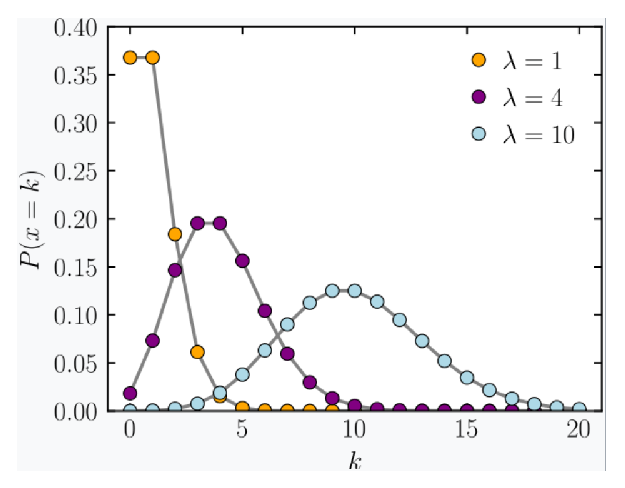
\includegraphics[width=0.25\paperwidth]{images/dist_poisson} \includegraphics[width=0.25\paperwidth]{images/cdf_poisson}
\par\end{centering}
\caption{Poisson PMF (left) CDF (right)}
\end{figure}

\end{enumerate}
\begin{enumerate}[resume]
\item Random sample $X_{1},...,X_{n}\sim\text{Pois}(\lambda)$ where $\lambda$
is target parameter: exponential family? sufficient statistic? minimal
sufficient statistic? complete statistic? Fisher information? UMVUE?
\begin{enumerate}
\item \textbf{Exponential family} form: $\mathop{\stackrel[i=1]{n}{\prod}[x_{i}!]^{-1}}\cdot e^{-n\lambda}\exp\left(\sum_{i=1}^{n}x_{i}\log\lambda\right)$
\item \textbf{Minimal sufficient and complete statistic}: $\sum_{i=1}^{n}X_{i}$
\item \textbf{Fisher information}: $\frac{n}{\lambda}$
\item \textbf{UMVUE}: $\frac{1}{n}\sum_{i=1}^{n}X_{i}$
\item \textbf{MLE} $\hat{\lambda}=\frac{1}{n}\sum_{i=1}^{n}X_{i}$
\end{enumerate}
\item \textbf{Conjugate prior }of $\lambda$?

$X|\lambda\sim\text{Pois}(\lambda)$

$\lambda\sim\text{Gamma}(\alpha,\beta)$

Posterior distribution $\lambda|(X=x)\sim\text{Gamma}(\alpha+\mathop{\sum_{i=1}^{n}x_{i}},\frac{1}{n+\frac{1}{\beta}})$

Note, above is if Gamma $pdf$ is written as $f(x)=\frac{1}{\Gamma(\alpha)\beta^{\alpha}}x^{\alpha-1}e^{-\frac{x}{\beta}}$

If Gamma $pdf$ is written as $f(x)=\frac{\beta^{\alpha}}{\Gamma(\alpha)}x^{\alpha-1}e^{-x\beta}$
then posterior distribution is written as $\lambda|(X=x)\sim\text{Gamma}(\alpha+\mathop{\sum_{i=1}^{n}x_{i}},n+\beta)$
\item \textbf{Related Distributions}

\begin{figure}[H]
\begin{centering}
\includegraphics[width=0.5\paperwidth]{images/poisson}
\par\end{centering}
\caption{Poisson and related distributions}
\end{figure}

\begin{enumerate}
\item \textbf{Additive property}
\begin{enumerate}
\item For $X_{i}\overset{ind}{\sim}\text{Pois}(\lambda_{i})$, then $\sum_{i=1}^{k}X_{i}\sim\text{Pois}(\sum_{i=1}^{k}\lambda_{i})$
\end{enumerate}
\item \textbf{Relation to Binomial} distribution
\begin{enumerate}
\item If $X\sim\text{Pois}(\lambda_{x})$ and $Y\sim\text{Pois}(\lambda_{y})$
and they are independent, then $X|X+Y=n\sim\text{Binom}\left(n,\frac{\lambda_{x}}{\lambda_{x}+\lambda_{y}}\right)$
\end{enumerate}
\item \textbf{Normal Approximation} (via CLT)
\begin{enumerate}
\item If $X\sim\text{Pois}(\lambda)$ then $Z=\frac{X-\lambda}{\sqrt{\lambda}}\overset{d}{\rightarrow}N(0,1)$
for $n\rightarrow\infty$
\end{enumerate}
\end{enumerate}
\item Example problems and key steps
\end{enumerate}
\pagebreak{}

\subsection{Negative Binomial}

Let us say that $X$ is distributed $\text{NBin}(r,p)$. We know the
following: $X$ is the number of \textquotedblleft failures\textquotedblright{}
that we will have before we achieve our rth success. Our successes
have probability $p$.
\begin{enumerate}
\item \textbf{PMF, MGF, mean and variance} of $X\sim\text{NegBinom}(r,p)$
\begin{enumerate}
\item \textbf{PMF}: 
\[
f(x)={x+r-1 \choose x}p^{r}(1-p)^{x}
\]

\begin{center}
$x=0,1,...n$
\par\end{center}

\begin{center}
$0<p<1$
\par\end{center}
\item \textbf{MGF}: $M_{X}(t)=\left(\frac{p}{1-(1-p)e^{t}}\right)^{r}$,
$t<-\log p$
\item \textbf{Mean and Variance}: 
\[
E[X]=\frac{r(1-p)}{p},\,\,Var(X)=\frac{r(1-p)}{p^{2}}
\]
\end{enumerate}
\begin{figure}[H]
\begin{centering}
\includegraphics[width=0.25\paperwidth]{images/dist_negbinomial} 
\par\end{centering}
\caption{Negative Binomial PMF}
\end{figure}

\item \textbf{Additive property}

If for $i=1,2,...,k$, $X_{i}\overset{ind}{\sim}\text{NegBinom}(r_{i},p)$,
then $\sum_{i=1}^{k}X_{i}\sim\text{NegBinom}(\sum_{i=1}^{k}r_{i},p)$
\end{enumerate}
\begin{enumerate}[resume]
\item Random sample $X_{1},...,X_{n}\overset{i.i.d}{\sim}\text{NegBinom}(r,p)$
where $p$ is target parameter and $r$ is known: exponential family?
sufficient statistic? minimal sufficient statistic? complete statistic?
Fisher information? UMVUE?
\begin{enumerate}
\item \textbf{Exponential family} form: $\mathop{\stackrel[i=1]{n}{\prod}{x_{i}+r-1 \choose x_{i}}}\cdot p^{nr}\exp\left(\sum_{i=1}^{n}x_{i}\log(1-p)\right)$
\item \textbf{Minimal sufficient and complete statistic}: $\sum_{i=1}^{n}X_{i}$
\item \textbf{Fisher information}: $\frac{nr}{p^{2}(1-p)}$
\item \textbf{UMVUE}: 
\begin{enumerate}
\item $\frac{1-p}{p}$: $\frac{\sum_{i=1}^{n}x_{i}}{nr}$
\item $p^{r}$: $P(X_{i}=0)$, $E(X_{i}=0|\sum_{i=1}^{n}X_{i})$, $E(\sum_{i=1}^{n}x_{i})=\frac{nr(1-p)}{p}$

$T=I_{(X_{i}=1)}(X_{i})$ where $E(T)=P(X_{i}=1)=p^{r}$. Let $S=\sum_{i=1}^{n}X_{i}$
and consider $E[T|S]$ (Rao Blackwell).

$E[T|S]=E[T=1|S=s]={\displaystyle \frac{p^{t}{s-t-1 \choose r-t-1}p^{r-t}(1-p)^{s-r}}{{s-1 \choose r-1}p^{r}(1-p)^{s-r}}=\frac{(s-t-1)!(r-1)!}{(s-1)!(r-t-1)!}}$
is UMVUE
\end{enumerate}
\end{enumerate}
\item \textbf{Conjugate prior} of $p$?

$X|p\sim\text{NegBinom}(r,p)$

$p\sim\text{beta}(\alpha,\beta)$.

\textbf{Posterior} distribution $p|(X=x)\sim\text{beta}(\alpha+nr,\beta+\sum_{i=1}^{n}x_{i})$
\item \textbf{Related Distributions}

\begin{figure}[H]
\begin{centering}
\includegraphics[width=0.5\paperwidth]{images/negbinomial}
\par\end{centering}
\caption{Negative Binomial and related distributions}
\end{figure}

\begin{enumerate}[resume]
\item If $X\sim\text{NegBinom}(r,p)$ for $r=1$, it becomes geometric distribution
with succss probability $p$
\item With $p=\frac{r}{r+\lambda}$, with $X\sim\text{NegBinom}(r,\frac{r}{r+\lambda})$,
then $X\overset{d}{\rightarrow}\text{Pois}(\lambda)$ for $r\rightarrow\infty$.
\end{enumerate}
\item \textbf{Example problems} and key steps
\end{enumerate}
\pagebreak{}

\subsection{Geometric{*}{*}{*}}

Let us say that $X$ is distributed $\text{Geom}(p)$. We know the
following: $X$ is the number of \textquotedblleft failures\textquotedblright{}
that we will achieve before we achieve our first success. Our successes
have probability $p$.

Number of Bernoulli trials before a success. (Negative binomial with
$r=1$)
\begin{enumerate}
\item \textbf{PMF, MGF, mean and variance} of $X\sim\text{Geom}(p)$
\begin{enumerate}
\item \textbf{PMF}:
\begin{enumerate}
\item $x$ trials before first success: 
\[
f(x)=p(1-p)^{x-1}
\]

\begin{center}
$x=1,2,...$
\par\end{center}

\begin{center}
$0<p<1$
\par\end{center}
\item $x$ failures before first success: 
\[
f(x)=p(1-p)^{x}
\]

\begin{center}
$x=0,1,2,...$; 
\par\end{center}

\begin{center}
$0<p<1$
\par\end{center}
\end{enumerate}
\item \textbf{CDF}: 
\begin{enumerate}
\item $x$ trials before first success: $F(t)=1-(1-p)^{t},\,\,t=1,2,...$
\item $x$ failures before first success: $F(t)=1-(1-p)^{t+1},\,\,t=0,1,2,...$
\end{enumerate}
\item \textbf{MGF}: $M_{X}(t)=\left(\frac{pe^{t}}{1-(1-p)e^{t}}\right)^{r}$,
$t<-\log(1-p)$
\item \textbf{Mean and Variance}: 
\begin{center}
$E[X]=\frac{1}{p}$, $Var(X)=\frac{(1-p)}{p^{2}}$ for $f(x)=p(1-p)^{x-1},\,\,x=1,2,...$
\par\end{center}

\begin{center}
$E[X]=\frac{1-p}{p}$, $Var(X)=\frac{(1-p)}{p^{2}}$ for $f(x)=p(1-p)^{x},\,\,x=0,1,2,...$
\par\end{center}

\end{enumerate}
\begin{figure}[H]
\begin{centering}
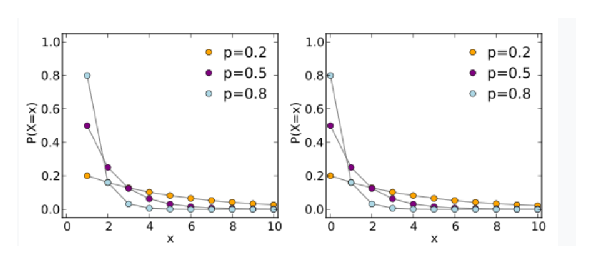
\includegraphics[width=0.25\paperwidth]{images/dist_geometric} 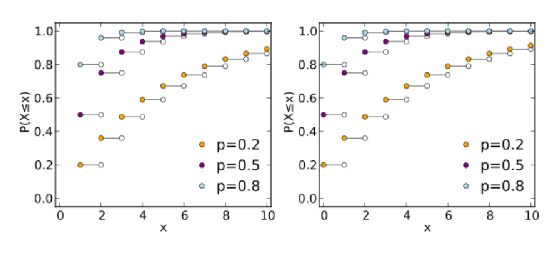
\includegraphics[width=0.25\paperwidth]{images/cdf_geometric}
\par\end{centering}
\caption{Geometric PMF (left) CDF (right)}
\end{figure}

\end{enumerate}
\begin{enumerate}[resume]
\item Random sample $X_{1},...,X_{n}\overset{i.i.d}{\sim}\text{Geom}(p)$
where $p$ is target parameter: exponential family? sufficient statistic?
minimal sufficient statistic? complete statistic? Fisher information?
UMVUE?
\begin{enumerate}[resume]
\item \textbf{Exponential family} form: $\left(\frac{p}{1-p}\right)^{n}\exp\left(\sum_{i=1}^{n}x_{i}\log(1-p)\right)$
for $f(x)=p(1-p)^{x-1},\,\,x=1,2,...$
\item \textbf{Minimal sufficient and complete statistic}: $\sum_{i=1}^{n}X_{i}$
\item \textbf{Fisher information}: $\frac{n}{p^{2}(1-p)}$ 
\item \textbf{UMVUE}: 
\begin{enumerate}[resume]
\item $\frac{1}{p}$: $\frac{\sum_{i=1}^{n}x_{i}}{n}$ for $f(x)=p(1-p)^{x-1},\,\,x=1,2,...$
\item $\frac{1-p}{p}$: $\frac{\sum_{i=1}^{n}x_{i}}{n}$ for $f(x)=p(1-p)^{x},\,\,x=0,1,2,...$
\end{enumerate}
\begin{enumerate}
\item $p$: $\sum_{i=1}^{n}x_{i}\sim\text{NegBin}(n,p)$ is sufficient and
complete, by L-S UMVUE is ${\displaystyle \frac{(n-1)}{(n-1+\sum_{i=1}^{n}x_{i})}}$

$E\left(\frac{(n-1)}{(n-1+n\bar{X})}\right)=\sum_{k=0}^{\infty}\frac{(n-1)}{(n-1+k)}{n+k-1 \choose k}p^{n}(1-p)^{k}=\sum_{k=0}^{\infty}\frac{(n-1)}{(n-1+k)}\frac{(n+k-1)!}{(n-1)!k!}p^{n}(1-p)^{k}$

$\sum_{k=0}^{\infty}\frac{(n+k-2)!}{(n-2)!k!}p^{n}(1-p)^{k}=p\sum_{k=0}^{\infty}{n+k-2 \choose k}p^{n-1}(1-p)^{k}=p$
\end{enumerate}
\end{enumerate}
\item \textbf{Conjugate prior} of $p$?

$X|p\sim\text{Geom}(p)$

$p\sim\text{beta}(\alpha,\beta)$.

Posterior distribution $p|(X=x)\sim\text{beta}(\alpha+n,\beta+\sum_{i=1}^{n}x_{i}-n)$
\item \textbf{Related Distributions}

\begin{figure}[H]
\begin{centering}
\includegraphics[width=0.4\paperwidth]{images/geometric}
\par\end{centering}
\caption{Geometric and related distributions}
\end{figure}

\begin{enumerate}
\item If $X\sim\text{Geom}(p)$ then $\sum_{i=1}^{r}X_{i}\sim\text{NegBinom}(r,p)$
\item If $X\sim\text{Geom}(p_{1})$ and $Y\sim\text{Geom}(p_{2})$ are independent,
and $Z=\min(X,Y)$, then $Z\sim\text{Geom}(1-[1-p_{1}][1-p_{2}])$
\end{enumerate}
\item \textbf{Example problems }and key steps
\end{enumerate}
\pagebreak{}

\subsection{Hypergeometric}

In a population of M desired objects and N undesired objects, x is
the number of \textquotedblleft successes\textquotedblright{} we will
have in a draw of K objects, without replacement. The draw of K objects
is assumed to be a simple random sample (all sets of K objects are
equally likely).
\begin{enumerate}
\item \textbf{PMF, MGF, mean and variance} of $X\sim\text{Hypergeometric}(N,M,K)$
\begin{enumerate}
\item \textbf{PMF}:

\[
P(X=x|N,M,K)=\dfrac{{M \choose x}{N-M \choose K-x}}{{N \choose K}}
\]
 
\begin{center}
$x=0,1,...,K$ and $\max(0,K+M-N)\leq x\leq\min(M,K)$
\par\end{center}

\begin{center}
$M\in\{0,1,2,...,N\},K\in\{0,1,2,...,N\}$, $N\in\{0,1,2...\}$
\par\end{center}
\item \textbf{MGF}: $M_{X}(t)=\frac{{N-M \choose K}\sideset{_{2}}{_{1}}F\left(-K,-M;N-M-K+1;e^{t}\right)}{{N \choose K}}$
\item \textbf{Mean and Variance}: 

\[
E[X]=\frac{KM}{N},\,\,Var(X)=\frac{KM}{N}\left(\frac{(N-M)(N-K)}{N(N-1)}\right)
\]

\end{enumerate}
\begin{figure}[H]
\begin{centering}
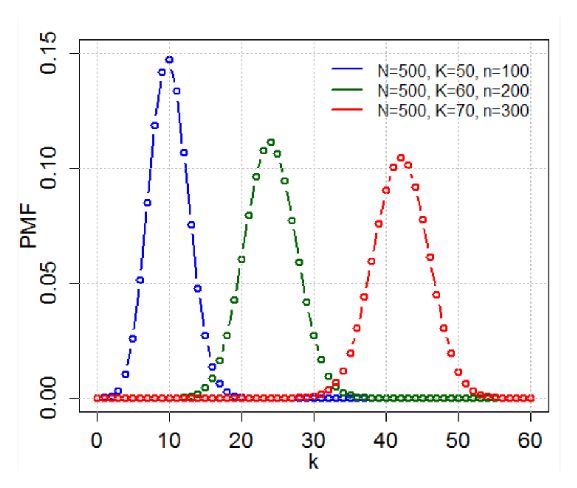
\includegraphics[width=0.25\paperwidth]{images/dist_hypergeometric}
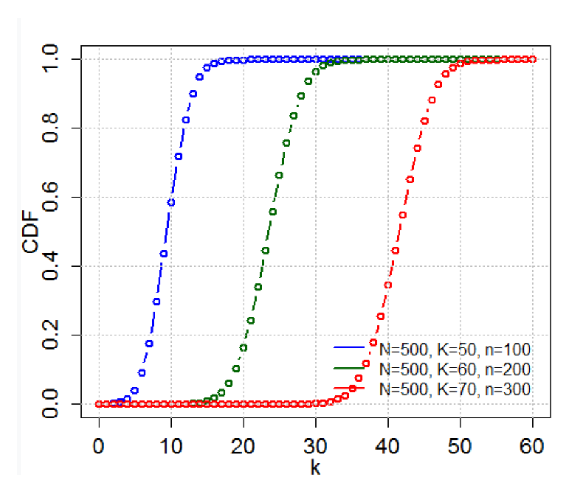
\includegraphics[width=0.25\paperwidth]{images/cdf_hypergeometric}
\par\end{centering}
\caption{Hypergeometric PMF (left) CDF (right)}
\end{figure}

\end{enumerate}
\begin{enumerate}[resume]
\item Random sample $X_{1},...,X_{n}\overset{i.i.d}{\sim}H\text{Geom}(N,M,K)$
where $p$ is target parameter: exponential family? sufficient statistic?
minimal sufficient statistic? complete statistic? Fisher information?
UMVUE?{*}{*}
\begin{enumerate}[resume]
\item Exponential family form: 
\item Minimal sufficient and complete statistic: {*}{*}
\item Fisher information: {*}{*}
\item UMVUE: 
\end{enumerate}
\item \textbf{Conjugate prior} of $p$?

$X|N,M,K\sim\text{HGeom}(N,M,K)$

$p\sim\text{BetaBin}(n,\alpha,\beta)$.

\textbf{Posterior} distribution $p|(X=x)\sim\text{BetaBin}($?)
\item \textbf{Related Distributions}

\begin{figure}[H]
\begin{centering}
\includegraphics[width=0.5\paperwidth]{images/hypergeometric}
\par\end{centering}
\caption{Hypergeometric and related distributions}
\end{figure}

If $X\sim\text{Hypergeometric}(N,M,K)$ and $p=\frac{M}{N}$
\begin{enumerate}
\item If $K=1$ then $X\sim\text{Ber}(p=\frac{M}{N})$
\item If $Y\sim\text{Bin}(n,p)$ then $Y$ models the number of successes
in the analagous sampling problem \emph{with} replacement. If $N$
and $M$ are large compared to $K$, and $p$ is not close to 0 or
1, then $X$ and $Y$ have similar distributions, i.e. $P(X\leq c)\approx P(Y\leq c)$.
\item If $K$ is large and $M$ and $N$ are large compared to $K$, and
$p$ is not close to $0$ or $1$, then $P(X\leq x)\approx\Phi\left(\frac{x-Kp}{\sqrt{Kp(1-p)}}\right)$
\end{enumerate}
\item \textbf{Example problems} and key steps
\end{enumerate}
\pagebreak{}

\section{Continuous Distributions}

\subsection{Continuous Uniform}

Let us say that $U$ is distributed $\text{Unif}(a,b)$. We know the
following: \textbf{Properties of the Uniform} For a Uniform distribution,
the probability of a draw from any interval within the support is
proportional to the length of the interval.
\begin{enumerate}
\item \textbf{PDF, CDF, MGF, mean and variance} of $X\sim\text{Unif}(a,b)$
\begin{enumerate}
\item \textbf{PDF}: 
\[
f(x)=\frac{1}{b-a}
\]

\begin{center}
$a\leq x\leq b$
\par\end{center}

\begin{center}
$a\in\mathbb{R},b\in\mathbb{R}$
\par\end{center}
\item \textbf{CDF}: $f(t)=\frac{x-a}{b-a}$

$a\leq t\leq b$

$a\in\mathbb{R},b\in\mathbb{R}$
\item \textbf{MGF}: $M_{X}(t)=\frac{e^{bt}-e^{at}}{(b-a)t}$
\item \textbf{Mean and Variance}: 
\[
E[X]=\frac{a+b}{2},\,\,Var(X)=\frac{(b-a)^{2}}{12}
\]
\end{enumerate}
\begin{figure}[H]
\begin{centering}
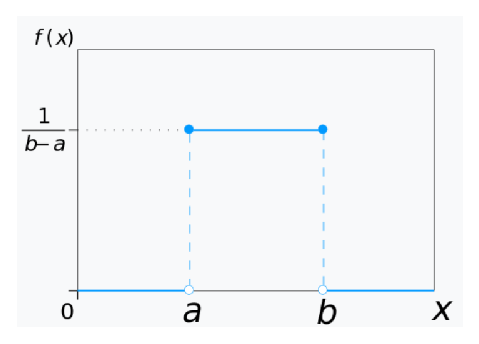
\includegraphics[width=0.25\paperwidth]{images/dist_uniform} 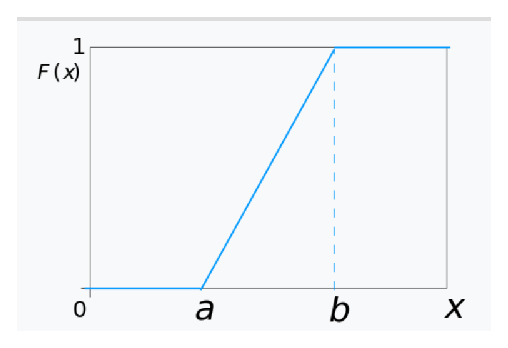
\includegraphics[width=0.25\paperwidth]{images/cdf_uniform}
\par\end{centering}
\caption{Uniform PDF (left) CDF (right)}
\end{figure}

\end{enumerate}
\begin{enumerate}[resume]
\item Random sample $X_{1},...,X_{n}\sim\text{Unif}(0,b)$ where $b$ is
target parameter: exponential family? sufficient statistic? minimal
sufficient statistic? complete statistic? Fisher information? UMVUE?
\begin{enumerate}[resume]
\item \textbf{Not exponential family}
\item \textbf{Scale family}: the standard distribution is $\text{Unif}(0,1)$
and $\frac{X_{i}}{b}\sim\text{Unif}(0,1)$ ($b$ is the scale parameter)
\item \textbf{Minimal sufficient and complete statistic}: $X_{(n)}$
\item \textbf{Fisher information}: $\frac{n}{b^{2}}$
\item \textbf{UMVUE}: $\frac{n+1}{n}X_{(n)}$ whose variance is $\frac{b^{2}}{n(n+2)}$
less than CRLB, indicating C-R inequality is not applicable for this
population. (read Casella example 7.3.13)
\end{enumerate}
\item Random sample $X_{1},...,X_{n}\sim\text{Unif}(a,b)$ where $a,b$
are target parameters: exponential family? sufficient statistic? minimal
sufficient statistic? complete statistic? Fisher information? UMVUE?
\begin{enumerate}[resume]
\item \textbf{Not exponential family}
\item \textbf{Scale family}: the standard distribution is $\text{Unif}(0,1)$
and $\frac{X_{i}-a}{b-a}\sim\text{Unif}(0,1)$ (a is the location
parameter and $b-a$ is the scale parameter)
\item \textbf{Minimal sufficient and complete statistic}: $(X_{(1)},X_{(n)})$.
\item \textbf{MLE} of $a$ is $X_{(1)}$ and \textbf{MLE} of $b$ is $X_{(n)}$.
\textbf{MLE} of $\theta=b-a$ is $\hat{\theta}=X_{(n)}-X_{(1)}$ by
invariance property of MLE.
\end{enumerate}
\item \textbf{Related Distributions}

\begin{figure}[H]
\begin{centering}
\includegraphics[width=0.5\paperwidth]{images/uniform}
\par\end{centering}
\caption{Uniform related distributions}
\end{figure}

\begin{enumerate}[resume]
\item If $X\sim\text{Unif}(a,b)$ then single order statistics (Casella
example 5.4.5): $\frac{X_{(j)}-a}{b-a}\sim\text{Beta}(j,n-j+1)${*}
\item If $X\sim\text{Unif}(0,1)$, then $-\lambda\log X\sim\text{EXP}(\lambda)$
($\lambda$ is scale parameter)
\item Bivariate order statistics (assuming $i<j$): $\left(\frac{X_{(i)}-a}{b-a},\frac{X_{(j)}-a}{b-a}\right)\sim\text{Dir}(i,j-i,n-j+1)$
(Casella exercise 4.40 for Dirichlet distribution)
\end{enumerate}
\item \textbf{Example problems }and key steps
\end{enumerate}
\pagebreak{}

\subsection{Gamma}

Let us say that $X$ is distributed $\text{Gamma}(a,\beta)$. We know
the following: You sit waiting for shooting stars, where the waiting
time for a star is distributed $\text{EXP}(\beta)$. You want to see
$n$ shooting stars before you go home. The total waiting time for
the $n$th shooting star is $\text{Gamma}(n,\beta)$.
\begin{enumerate}
\item \textbf{PDF, MGF, mean and variance} of $X\sim\text{Gamma}(\alpha,\beta)$,
$\alpha,\beta>0$, $\beta$ is the scale parameter. 
\begin{enumerate}
\item \textbf{PDF}: 
\[
f(x)=\frac{1}{\Gamma(\alpha)\beta^{\alpha}}x^{\alpha-1}e^{-\frac{x}{\beta}}
\]

\begin{center}
$x>0$
\par\end{center}

\begin{center}
$\alpha>0$, $\beta>0$
\par\end{center}
\item \textbf{MGF}: $M_{X}(t)=\left(1-\beta t\right)^{-\alpha}$, $t<\frac{1}{\beta}$
\item \textbf{Mean and Variance}: 
\[
E[X]=\alpha\beta,\,\,Var(X)=\alpha\beta^{2}
\]
\end{enumerate}
\begin{figure}[H]
\begin{centering}
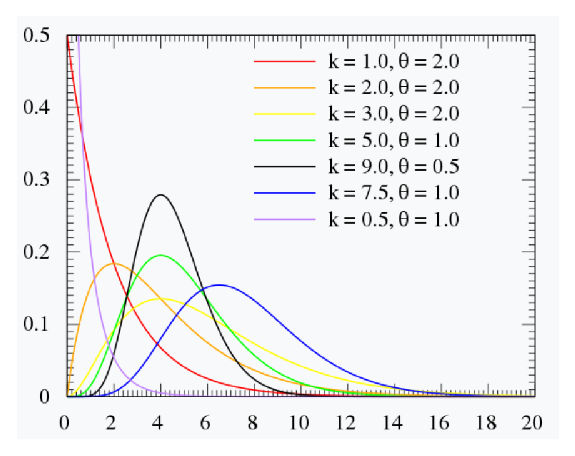
\includegraphics[width=0.25\paperwidth]{images/dist_gamma} 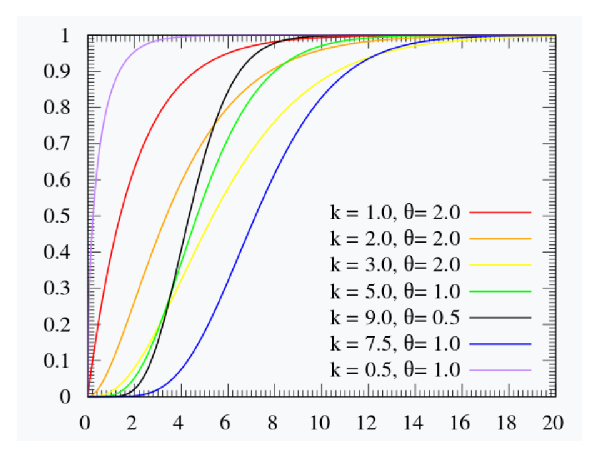
\includegraphics[width=0.25\paperwidth]{images/cdf_gamma}
\par\end{centering}
\caption{Gamma PDF (left) CDF (right)}
\end{figure}

\end{enumerate}
\begin{enumerate}[resume]
\item \textbf{Additivity and Scaling}
\begin{enumerate}[resume]
\item If $X_{i}\overset{ind}{\sim}\text{Gamma}(\alpha_{i},\beta)$, then
$\sum_{i=1}^{k}X_{i}\sim\text{Gamma}(\sum_{i=1}^{k}\alpha_{i},\beta)$
\item If $X\sim\text{Gamma}(\alpha,\beta)$ then $cX\sim\text{Gamma}(\alpha,c\beta)$
\end{enumerate}
\item Random sample $X_{1},...,X_{n}\overset{i.i.d}{\sim}\text{Gamma}(\alpha,\beta)$
where $\beta$ is target parameter and $\alpha$ is known: exponential
family? sufficient statistic? minimal sufficient statistic? complete
statistic? Fisher information? UMVUE?
\begin{enumerate}[resume]
\item \textbf{Exponential family} form: 
\[
\mathop{\stackrel[i=1]{n}{\prod}x_{i}^{\alpha-1}}\cdot\,\left(\Gamma(\alpha)\beta^{\alpha}\right)^{-1}\exp\left(-\frac{1}{\beta}\sum_{i=1}^{n}x_{i}\right)
\]
\item \textbf{Scale family}: the standard distribution is $\text{Gamma}(\alpha,1)$
and $\frac{X_{i}}{\beta}\sim\Gamma(\alpha,1)$
\item \textbf{Minimal sufficient and complete statistic}: $\sum_{i=1}^{n}X_{i}$
\item \textbf{Fisher information}: $\frac{n\alpha}{\beta^{2}}$
\item \textbf{UMVUE}: $\frac{1}{n\alpha}\sum_{i=1}^{n}X_{i}$
\end{enumerate}
\item \textbf{Related Distributions}

\begin{figure}[H]
\begin{centering}
\includegraphics[width=0.5\paperwidth]{images/gamma}
\par\end{centering}
\caption{Gamma related distributions}
\end{figure}

\begin{enumerate}[resume]
\item If $X\sim\text{Gamma}(\alpha,\beta)$, for $\alpha=1$, $X\sim\text{Exp}(\beta)$
\item \textbf{Pivot: }If $X\sim\text{Gamma}(\alpha,\beta)$, for $\alpha=\frac{n}{2}$,
$\beta=2$, $X\sim\chi_{n}^{2}${*}
\item If $X\sim\text{Gamma}(\alpha,\theta)$ and $Y\sim\text{Gamma}(\beta,\theta)$
are independent, then $Z=\frac{X}{X+Y}\sim\text{Beta}(\alpha,\beta)$
\item If $X\sim\text{Gamma}(\alpha,\beta)$, for large $\alpha$ $X$ converges
in distribution to $\text{N}(\alpha\beta,\alpha\beta^{2})$
\item If $X\sim\text{Gamma}(\alpha,\beta)$, then $\frac{1}{X}\sim\text{InvGamma}(\alpha,\frac{1}{\beta})$ 
\end{enumerate}
\item \textbf{Example problems} and key steps
\begin{enumerate}[resume]
\item \textbf{Example} You are at a bank, and there are 3 people ahead of
you. The serving time for each person is Exponential with mean 2 minutes.
Only one person at a time can be served. The distribution of your
waiting time until it\textquoteright s your turn to be served is $\text{Gamma}(3,12)$.
\end{enumerate}
\item Other notes
\begin{enumerate}[resume]
\item Gamma is sometimes considered the continuous analog of the negative
binomial distribution
\end{enumerate}
\end{enumerate}
\pagebreak{}

\subsubsection{Inverse Gamma}

If $X\sim\text{Gamma}(\alpha,\beta)$, then $\frac{1}{X}\sim\text{InvGamma}(\alpha,\frac{1}{\beta})$ 
\begin{enumerate}
\item \textbf{PDF, CDF,MGF, mean and variance} of $X\sim\text{InvGamma}(\alpha,\beta)$,
$\alpha,\beta>0$, $\beta$ is the scale parameter. 
\begin{enumerate}
\item \textbf{PDF}: 
\[
f(x)=\frac{\beta^{\alpha}}{\Gamma(\alpha)}(x)^{-(\alpha+1)}e^{-\frac{\beta}{x}}
\]

\begin{center}
$x>0$
\par\end{center}

\begin{center}
$\alpha>1$, $\beta>0$
\par\end{center}
\item \textbf{CDF:}
\end{enumerate}
\[
\frac{\Gamma(\alpha,\frac{\beta}{x})}{\Gamma(\alpha)}
\]

\begin{enumerate}
\item \textbf{MGF}: DNE
\item \textbf{Mean and Variance}: 
\[
E[X]=\frac{\beta}{\alpha-1},\,\,Var(X)=\frac{\beta^{2}}{(\alpha-1)^{2}(\alpha-2)}\,\,\,\alpha>2
\]
 
\end{enumerate}
\begin{figure}[H]
\begin{centering}
\includegraphics[width=0.25\paperwidth]{images/dist_invgamma} \includegraphics[width=0.25\paperwidth]{images/cdf_invgamma}
\par\end{centering}
\caption{Inverse Gamma PDF (left) CDF (right)}
\end{figure}

\end{enumerate}
\begin{enumerate}[resume]
\item \textbf{Scaling}
\begin{enumerate}[resume]
\item If $X\sim\text{InvGamma}(\alpha,\beta)$ then $cX\sim\text{Gamma}(\alpha,c\beta)$
for $c>0$
\end{enumerate}
\item Random sample $X_{1},...,X_{n}\overset{i.i.d}{\sim}\text{Gamma}(\alpha,\beta)$
where $\beta$ is target parameter and $\alpha$ is known: exponential
family? sufficient statistic? minimal sufficient statistic? complete
statistic? Fisher information? UMVUE?
\begin{enumerate}[resume]
\item \textbf{Exponential family} form: 
\[
\mathop{\stackrel[i=1]{n}{\prod}x_{i}^{-(\alpha+1)}}\cdot\,\left(\frac{\beta^{\alpha}}{\Gamma(\alpha)}\right)\exp\left(-\beta\sum_{i=1}^{n}\frac{1}{x_{i}}\right)
\]
\item \textbf{Scale family}: the standard distribution is $\text{InvGamma}(\alpha,1)$
\item \textbf{Minimal sufficient and complete statistic}: $\sum_{i=1}^{n}\frac{1}{X_{i}}$
\item \textbf{Fisher information}: $TBD$
\item \textbf{UMVUE}: $TBD$
\end{enumerate}
\item \textbf{Related Distributions}
\begin{enumerate}[resume]
\item If $X\sim\text{Gamma}(\alpha,\beta)$, then $\frac{1}{X}\sim\text{InvGamma}(\alpha,\frac{1}{\beta})$ 
\item If $X\sim\text{InvGamma}(1,c)$ then $\frac{1}{X}\sim EXP(c)$ 
\end{enumerate}
\end{enumerate}
\pagebreak{}

\subsection{Normal}
\begin{enumerate}
\item \textbf{PDF, MGF, mean and variance }of $X\sim N(\mu,\sigma^{2})$
\begin{enumerate}
\item \textbf{PDF}: 
\[
f(x)=\frac{1}{\sqrt{2\pi\sigma^{2}}}e^{-\frac{(x-\mu)^{2}}{2\sigma^{2}}}
\]

\begin{center}
$-\infty<x<\infty$
\par\end{center}

\begin{center}
$-\infty<\mu<\infty$
\par\end{center}

\begin{center}
$\sigma>0$
\par\end{center}
\item \textbf{MGF}: $M_{X}(t)=\exp(\mu t+\frac{\sigma^{2}t^{2}}{2})$
\item \textbf{Mean and Variance}: 
\[
E[X]=\mu,\,\,Var(X)=\sigma^{2}
\]
\end{enumerate}
\begin{figure}[H]
\begin{centering}
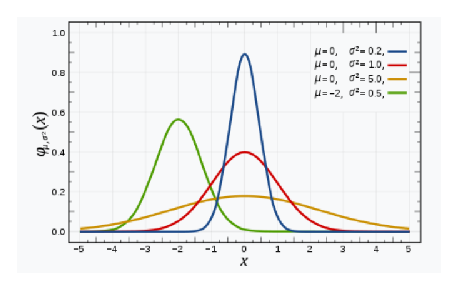
\includegraphics[width=0.25\paperwidth]{images/dist_normal} 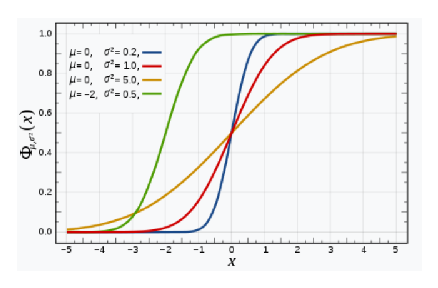
\includegraphics[width=0.25\paperwidth]{images/cdf_normal}
\par\end{centering}
\caption{Normal PDF (left) CDF (right)}
\end{figure}

\end{enumerate}
\begin{enumerate}[resume]
\item \textbf{Linearity} and \textbf{additivity}
\begin{enumerate}[resume]
\item If $X\sim N(\mu,\sigma^{2})$, then $aX+b\sim N(a\mu+b,a^{2}\sigma^{2})$
\item If $X_{1}\sim N(\mu_{1},\sigma_{1}^{2})$ and $X_{2}\sim N(\mu_{2},\sigma_{2}^{2})$
and $X_{1},X_{2}$ are independent, then $X_{1}\pm X_{2}\sim N(\mu_{1}\pm\mu_{2},\sigma_{1}^{2}+\sigma_{2}^{2})$.
\end{enumerate}
\item Population $\text{\ensuremath{X_{1}},...,\ensuremath{X_{n}\overset{i.i.d}{\sim}}}N(\mu,\sigma_{0}^{2})$
($\mu$ is unknown and $\sigma_{0}^{2}$ is known)
\begin{enumerate}[resume]
\item \textbf{Exponential family} form: $(2\pi\sigma_{0}^{2})^{-\frac{n}{2}}\exp\left(-n\frac{\mu^{2}}{2\sigma_{0}^{2}}\right)\exp\left(-\sum_{i=1}^{n}\frac{x_{i}^{2}}{2\sigma_{0}^{2}}\right)\exp\left(\frac{\mu}{\sigma_{0}^{2}}\sum_{i=1}^{n}x_{i}\right)$
\item \textbf{Location family}: the standard distribution is $N(0,\sigma_{0}^{2})$
and $X_{i}-\mu\sim N(0,\sigma_{0}^{2})$.
\item \textbf{Minimal sufficient and complete statistic}: $\sum_{i=1}^{n}X_{i}$
\item \textbf{Fisher information}: $\frac{n}{\sigma_{0}^{2}}$
\item \textbf{UMVUE}: $\frac{1}{n}\sum_{i=1}^{n}X_{i}$
\item \textbf{Conjugate prior }of $\mu\sim N(a,b^{2})$
\end{enumerate}
$X|\mu\sim N(\mu,\sigma_{0}^{2})$

$\mu\sim N(a,b^{2})$

\textbf{Posterior }distribution $\mu|(X=x)\sim N\left(\left(\frac{a}{b^{2}}+\frac{n\bar{x}}{\sigma_{0}^{2}}\right)\left(\frac{b^{2}\sigma_{0}^{2}}{\sigma_{0}^{2}+nb^{2}}\right),\left(\frac{b^{2}\sigma_{0}^{2}}{\sigma_{0}^{2}+nb^{2}}\right)\right)$
\item Population $\text{\ensuremath{X_{1}},...,\ensuremath{X_{n}\overset{i.i.d}{\sim}}}N(0,\sigma^{2})$
($\sigma^{2}$ is unknown)
\begin{enumerate}[resume]
\item \textbf{Exponential family }form: 
\[
(2\pi\sigma^{2})^{-\frac{n}{2}}\exp\left(-\frac{1}{2\sigma^{2}}\sum_{i=1}^{n}x_{i}^{2}\right)
\]
\item \textbf{Scale family}: the standard distribution is $N(0,1)$ and
$\frac{X_{i}}{\sigma}\sim N(0,1)$.
\item \textbf{Minimal sufficient and complete statistic}: $\sum_{i=1}^{n}X_{i}^{2}$
\item \textbf{Fisher information}: $\frac{n}{2\sigma^{4}}$
\item \textbf{UMVUE}: $\frac{1}{n}\sum_{i=1}^{n}X_{i}^{2}$
\item \textbf{Conjugate prior }of $\frac{1}{\sigma^{2}}\sim\text{Gamma}(\alpha,\beta)$
\end{enumerate}
$X|\sigma^{2}\sim N(0,\sigma^{2})$

$\sigma^{2}\sim\text{InvGamma}(\alpha,\beta)$

\textbf{Posterior }distribution $\sigma^{2}|(X=x)\sim\text{InvGamma}\left(\alpha+\frac{n}{2},\frac{1}{\frac{1}{2}\sum_{i=1}^{n}X_{i}^{2}+\frac{1}{\beta}}\right)$
\item Population $\text{\ensuremath{X_{1}},...,\ensuremath{X_{n}\overset{i.i.d}{\sim}}}N(\mu,\sigma^{2})$
($\mu$ is unknown and $\sigma^{2}$ is unknown)
\begin{enumerate}[resume]
\item \textbf{Exponential family }form: 
\[
(2\pi\sigma^{2})^{-\frac{n}{2}}\exp\left(-n\frac{\mu^{2}}{2\sigma^{2}}\right)\exp\left(\frac{\mu}{\sigma^{2}}\sum_{i=1}^{n}x_{i}-\frac{1}{2\sigma^{2}}\sum_{i=1}^{n}x_{i}^{2}\right)
\]
\item \textbf{Location-Scale family}: the standard distribution is $N(0,1)$
and $\frac{X_{i}-\mu}{\sigma}\sim N(0,1)$.
\item \textbf{Minimal sufficient and complete statistic}: $\left(\sum_{i=1}^{n}X_{i},\sum_{i=1}^{n}X_{i}^{2}\right)$
\item \textbf{Fisher information}: $I=\text{diag}(\frac{n}{\sigma^{2}},\frac{n}{2\sigma^{4}})$
\item \textbf{UMVUE}: $\left(\bar{X},S^{2}\right)$
\item \textbf{Conjugate prior }of $\mu\sim N(a,b^{2})$, $\sigma^{2}\sim\text{InvGamma}(\alpha,\beta)$
or $\frac{1}{\sigma^{2}}\sim\text{Gamma}(\alpha,\beta)$
\end{enumerate}
\item \textbf{Related Distributions}

\begin{figure}[H]
\begin{centering}
\includegraphics[width=0.5\paperwidth]{images/normal}
\par\end{centering}
\caption{Normal related distributions}
\end{figure}

\begin{enumerate}[resume]
\item For $X_{1},...,X_{n}\overset{i.i.d}{\sim}N(0,1)$, $\sum_{i=1}^{n}X_{i}^{2}\sim\chi_{n}^{2}$
\item For $X_{1},...,X_{n}\overset{i.i.d}{\sim}N(\mu,\sigma^{2})$:
\begin{enumerate}[resume]
\item $\bar{X}\sim N(\mu,\frac{\sigma^{2}}{n})$
\item $\frac{S^{2}}{\sigma^{2}}\sim\chi_{n-1}^{2}$ where $S^{2}=\frac{1}{n-1}\mathop{\sum_{i=1}^{n}(X_{i}-\bar{X})^{2}}$
\item $\bar{X}$ and $S^{2}$ are independent and $\frac{\bar{X}-\mu}{\sqrt{S^{2}/n}}\sim t_{n-1}$
\end{enumerate}
\item If $Z\sim N(0,1)$, $Y\sim\chi_{n}^{2}$ and they are independent,
then $X=\frac{Z}{\sqrt{Y/n}}\sim t_{n}$
\item If $Y\sim\chi_{n}^{2}$ , $Z\sim\chi_{m}^{2}$ and they are independent,
then $X=\frac{Y}{Z}\sim F_{n,m}$
\item If $X\sim N(\mu,\sigma^{2})$, then $\exp(X)\sim\log N(\mu,\sigma^{2})$
\item If $X_{1}\sim N(0,1)$ and $X_{2}\sim N(0,1)$ are independent then
$\frac{X_{1}}{X_{2}}\sim\text{Cauchy}(0,1)$
\end{enumerate}
\item \textbf{Example problems }and key steps
\end{enumerate}
\pagebreak{}

\subsection{Exponential}

Let us say that $X$ is distributed $\text{EXP}(\beta)$. We know
the following: You\textquoteright re sitting on an open meadow right
before the break of dawn, wishing that airplanes in the night sky
were shooting stars, because you could really use a wish right now.
You know that shooting stars come on average every 15 minutes, but
a shooting star is not \textquotedblleft due\textquotedblright{} to
come just because you\textquoteright ve waited so long. Your waiting
time is memoryless; the additional time until the next shooting star
comes does not depend on how long you\textquoteright ve waited already.
\begin{enumerate}
\item \textbf{PDF, CDF, MGF, mean and variance }of $X\sim\text{Exp}(\beta)$,
$\beta>0$
\begin{enumerate}
\item \textbf{PDF}: 
\[
f(x)=\frac{1}{\beta}e^{-\frac{x}{\beta}}
\]

\begin{center}
$x>0$
\par\end{center}
\item \textbf{CDF}: $f(x)=(1-e^{-\frac{x}{\beta}})\cdot I_{[0,\infty)}(x)$
\item \textbf{MGF}: $M_{X}(t)=$$(1-\beta t)^{-1}$
\item \textbf{Mean and Variance}: 
\[
E[X]=\beta,\,\,Var(X)=\beta^{2}
\]
\end{enumerate}
\begin{figure}[H]
\begin{centering}
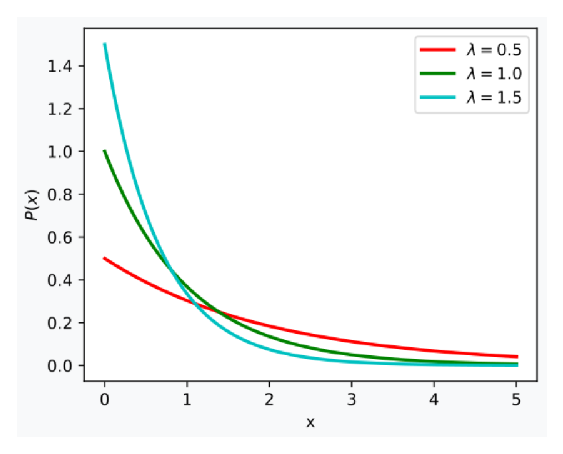
\includegraphics[width=0.25\paperwidth]{images/dist_exponential}
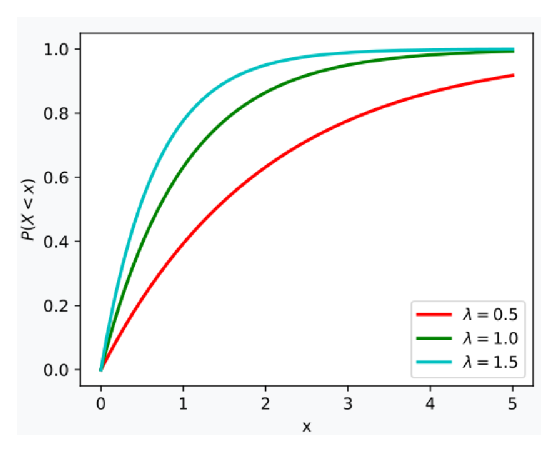
\includegraphics[width=0.25\paperwidth]{images/cdf_exponential}
\par\end{centering}
\caption{Exponential PDF (left) CDF (right)}
\end{figure}

\end{enumerate}
\begin{enumerate}[resume]
\item Random sample $X_{1},...,X_{n}\sim\text{Exp}(\beta)$ where $\beta$
is target parameter: exponential family? sufficient statistic? minimal
sufficient statistic? complete statistic? Fisher information? UMVUE?
\begin{enumerate}[resume]
\item \textbf{Exponential family}: 
\[
\left(\frac{1}{\beta}\right)^{n}\exp\left(-\frac{1}{\beta}\sum_{i=1}^{n}x_{i}\right)
\]
\item \textbf{Scale family}: The standard distribution is $\text{Exp}(1)$
and $\frac{X_{i}}{\beta}\sim\text{Exp}(1)$
\item \textbf{Minimal sufficient and complete statistic}: $\sum_{i=1}^{n}X_{i}$
\item \textbf{Fisher information}: $\frac{n}{\beta^{2}}$
\item \textbf{UMVUE}: $\frac{1}{n}\sum_{i=1}^{n}X_{i}$
\end{enumerate}
\item \textbf{Related Distributions}

\begin{figure}[H]
\begin{centering}
\includegraphics[width=0.5\paperwidth]{images/exponential}
\par\end{centering}
\caption{Exponential and related distributions}
\end{figure}

\begin{itemize}
\item If $X\sim\text{Laplace}(\mu,\frac{1}{\beta})$, then |$X-\mu|\sim\text{Exp}(\beta)$
(Laplace is double exponential)
\item $\lambda_{1}X_{1}-\lambda_{2}X_{2}\sim\text{Laplace}(0,1)${*}
\item If $X\sim\text{Pareto}(1,\lambda)$, then $\log(X)\sim\text{Exp}(\lambda)$
\item If $X_{i}\sim\text{Unif}(0,1)$, then $\underset{n\rightarrow\infty}{\lim}n\min(X_{1},...,X_{n})\sim\text{Exp}(1)${*}
\item Limit of a scaled Beta distribution $\underset{n\rightarrow\infty}{\lim}n\text{Beta}(1,n)\sim\text{Exp}(1)$
\end{itemize}
If $X\sim\text{Exp}(\lambda)$ and $X_{i}\sim\text{Exp}(\lambda_{i})$
\begin{itemize}
\item $kX\sim\text{Exp}\left(\frac{\lambda}{k}\right)$, closure under scaling
by a positive factor{*}
\item $ke^{x}\sim\text{Pareto}\left(k,\lambda\right)$
\item $e^{-X}\sim\text{Beta}\left(\lambda,1\right)$
\item $\sqrt{X}\sim\text{Rayleigh}\left(\frac{1}{\sqrt{2\lambda}}\right)$
\item $X\sim\text{Weibull}\left(\frac{1}{\lambda},1\right)$
\item $X^{2}\sim\text{Weibull}\left(\frac{1}{\lambda^{2}},\frac{1}{2}\right)$
\item $\min(X_{1},...,X_{n})\sim\text{Exp}(\lambda_{1},...,\lambda_{n})$
\end{itemize}
If also $\lambda_{i}=\lambda$
\begin{itemize}
\item $\sum_{i=1}^{k}X_{i}\sim\text{Gamma}(k,\lambda)$ or if $\beta$ parameter
then $\sim\text{Gamma}(k,\frac{1}{\beta})${*}
\begin{itemize}
\item $X\sim\text{Exp}(\beta)$ is equivalent to $X\sim\text{Gamma}(1,\beta)$
\end{itemize}
\item T=$\sum_{i=1}^{n}X_{i}$, then $2\lambda T\sim\chi_{2n}^{2}${*}
\item $X_{i}-X_{j}\sim\text{Laplace}(0,\lambda^{-1})$
\end{itemize}
If also $X_{i}$ are independent, then
\begin{itemize}
\item $\frac{X_{i}}{X_{i}+X_{j}}\sim\text{Unif}(0,1)${*}
\item $Z=\frac{\lambda_{i}X_{i}}{\lambda_{j}X_{j}}$has $pdf$ $f_{Z}(z)=\frac{1}{(z+1)^{2}}$.
This can be used as a confidence interval for $\frac{\lambda_{i}}{\lambda_{j}}$
\end{itemize}
If also $\lambda=\frac{1}{2}$ then $X\sim\chi_{2}^{2}$, a chi squared
distribution with two degrees of freedom, hence{*}
\begin{itemize}
\item $\text{Exp}(\lambda)=\frac{1}{2\lambda}\text{Exp}(\frac{1}{2})\sim\frac{1}{2\lambda}\chi_{2}^{2}$
so $\sum_{i=1}^{n}\text{Exp}(\lambda)\sim\frac{1}{2\lambda}\chi_{2}^{2}${*}
\item If $X\sim\text{Exp}(\frac{1}{\lambda})$ and $Y|X\sim\text{Pois}(X)$
then $Y\sim\text{Geom}(\frac{1}{1+\lambda})$
\end{itemize}
\item \textbf{Example problems} and key steps
\begin{enumerate}[resume]
\item \textbf{Example} The waiting time until the next shooting star is
distributed $\text{EXP}(4)$ hours. Here $\beta=4$ is the rate parameter,
since shooting stars arrive at a rate of 1 per 1/4 hour on average.
The expected time until the next shooting star is $1/\beta=1/4$ hour.
\item \textbf{Memorylessness} The Exponential Distribution is the only continuous
memoryless distribution. The memoryless property says that for $X\sim\text{EXP}(\lambda)$and
any positive numbers $s$ and $t$, 
\[
P(X>s+t|X>s)=P(X>t)
\]
 Equivalently, 
\[
X-a|(X>a)\sim\text{EXP}(\lambda)
\]
For example, a product with an $\text{EXP}(\lambda)$ lifetime is
always \textquotedblleft as good as new\textquotedblright{} (it doesn\textquoteright t
experience wear and tear). Given that the product has survived a years,
the additional time that it will last is still $\text{EXP}(\lambda)$.
\end{enumerate}
\end{enumerate}
\pagebreak{}

\subsection{Beta}
\begin{enumerate}
\item \textbf{PDF, MGF, mean and variance }of $X\sim\text{Beta}(\alpha,\beta)$,
$\alpha,\beta>0$, $\alpha,\beta$ are shape parameters. 
\begin{enumerate}
\item \textbf{PDF}: 
\[
f(x)=\frac{\Gamma(\alpha+\beta)}{\Gamma(\alpha)\Gamma(\beta)}x^{\alpha-1}(1-x)^{\beta-1}=\frac{x^{\alpha-1}(1-x)^{\beta-1}}{\text{B}(\alpha,\beta)}
\]

\begin{center}
$1>x>0$
\par\end{center}

\begin{center}
$\alpha>0$, $\beta>0$
\par\end{center}
\item \textbf{Mean and Variance}: 
\[
E[X]=\frac{\alpha}{\alpha+\beta},\,\,Var(X)=\frac{\alpha\beta}{(\alpha+\beta)^{2}(\alpha+\beta+1)}
\]
\end{enumerate}
\begin{figure}[H]
\begin{centering}
\includegraphics[width=0.25\paperwidth]{images/dist_beta} 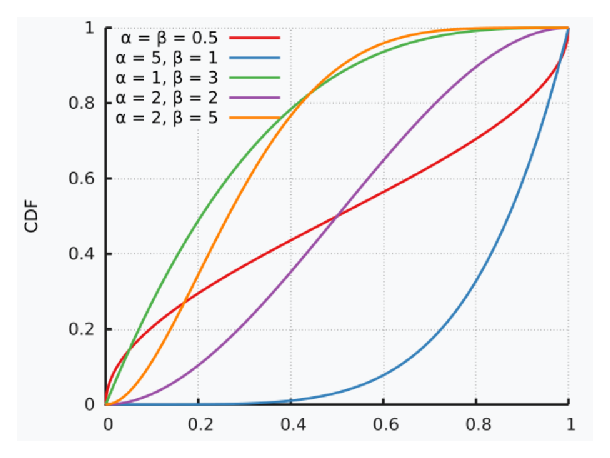
\includegraphics[width=0.25\paperwidth]{images/cdf_beta}
\par\end{centering}
\caption{Beta PDF (left) CDF (right)}
\end{figure}

\end{enumerate}
\begin{enumerate}[resume]
\item Random sample $X_{1},...,X_{n}\overset{i.i.d}{\sim}\text{Beta}(\alpha,\beta)$
where $\alpha,\beta$ are target parameters: exponential family? sufficient
statistic? minimal sufficient statistic? complete statistic? Fisher
information? UMVUE?
\begin{enumerate}[resume]
\item \textbf{Exponential family} form: 
\[
\exp\left[(\alpha-1)\sum_{i=1}^{n}\log x_{i}+(\beta-1)\sum_{i=1}^{n}\log(1-x_{i})+n\log\frac{\Gamma(\alpha+\beta)}{\Gamma(\alpha)\Gamma(\beta)}\right]
\]
\item \textbf{Minimal sufficient and complete statistic}: $T=\left(\sum_{i=1}^{n}\log X_{i},\sum_{i=1}^{n}\log(1-X_{i})\right)$
\item \textbf{Conjugate prior }to the Binomial

$X|p\sim\text{Bin}(n,p)$

$p\sim\text{Beta}(a,b)$

\textbf{Posterior} distribution: $p|(X=x)\sim\text{Beta}(a+x,b+n-x)$ 
\item For $\beta$ known, the\textbf{ MLE} of $\alpha$ $\sum_{i=1}^{n}\log X_{i}$
\item For $\alpha$ known, the\textbf{ MLE} of $\beta$ \textbf{$\boldsymbol{TBD****}$}
\end{enumerate}
\item \textbf{Related Distributions}

\begin{figure}[H]
\begin{centering}
\includegraphics[width=0.5\paperwidth]{images/beta}
\par\end{centering}
\caption{Beta related distributions}
\end{figure}

\begin{enumerate}[resume]
\item If $X\sim\text{Beta}(\alpha,\beta)$ then $1-X\sim\text{Beta}(\beta,\alpha)$
\item \textbf{Pivot: }If $X\sim\text{Beta}(\frac{n}{2},\frac{m}{2})$ with
$n>0,m>0$, then $\frac{mX}{n(1-X)}\sim F(n,m)$
\item If $X\sim\text{Beta}(\alpha,1)$ then $-\ln(X)\sim\text{EXP}(\alpha)$
\item For large $n$, if $X_{n}\sim\text{Beta}(n\alpha,n\beta)$ then $\sqrt{n}(\bar{X_{n}}-\frac{a}{a+\beta})\overset{d}{\rightarrow}N(0,\frac{a\beta}{(a+\beta)^{3}})$,
or similarly $\text{Beta}(n\alpha,n\beta)\overset{d}{\rightarrow}N(\frac{a}{a+\beta},\frac{a\beta}{(a+\beta)^{3}})$
\item If $X\sim\chi_{\alpha}^{2}$ and $Y\sim\chi_{\beta}^{2}$ are independent,
then $\frac{X}{X+Y}\sim\text{Beta}(\frac{\alpha}{2},\frac{\beta}{2})$
\item If $X\sim\text{Unif}(0,1)$ and $\alpha>0$ then $X^{\frac{1}{\alpha}}\sim\text{Beta}(\alpha,1)$
\item If $X\sim\text{Unif}(a,b)$ then single order statistics (Casella
example 5.4.5): $\frac{X_{(j)}-a}{b-a}\sim\text{beta}(j,n-j+1)${*}
\item If $X\sim\text{Gamma}(\alpha,\theta)$ and $Y\sim\text{Gamma}(\beta,\theta)$
are independent, then $Z=\frac{X}{X+Y}\sim\text{Beta}(\alpha,\beta)${*}
\item If $X\sim\text{Cauchy}(0,1)$ then $\frac{1}{1+X^{2}}\sim\text{Beta}(\frac{1}{2},\frac{1}{2})$
\end{enumerate}
\item \textbf{Example problems }and key steps
\begin{itemize}
\item Determine a minimal sufficient statistic if $\alpha=2\beta$

$\exp\left[(2\beta-1)\sum_{i=1}^{n}\log x_{i}+(\beta-1)\sum_{i=1}^{n}\log(1-x_{i})+n\log\frac{\Gamma(3\beta)}{\Gamma(2\beta)\Gamma(\beta)}\right]$ 

$=\exp\left[\sum_{i=1}^{n}\log x_{i}+(\beta-1)\sum_{i=1}^{n}\log x_{i}^{2}(1-x_{i})+n\log\frac{\Gamma(3\beta)}{\Gamma(2\beta)\Gamma(\beta)}\right]$, 

which is exponential family with minimal sufficient statistic $\sum_{i=1}^{n}\log x_{i}^{2}(1-x_{i})=2T_{1}+T_{2}$
where $T=\left(\sum_{i=1}^{n}\log X_{i},\sum_{i=1}^{n}\log(1-X_{i})\right)$
\item Determine a minimal sufficient statistic if $\alpha=\beta^{2}$

$p_{\beta}(x)=\exp\left[(\beta^{2}-1)T_{1}(x)+(\beta-1)T_{2}(x)+n\log\frac{\Gamma(\beta+\beta^{2})}{\Gamma(\beta)\Gamma(\beta^{2})}\right]$
use Lehmann Scheffe to show min sufficient that $T(x)=T(y)$
\end{itemize}
\item \textbf{Other notes}
\end{enumerate}
\pagebreak{}

\subsection{Log-normal{*}}

In probability theory, a log-normal (or lognormal) distribution is
a continuous probability distribution of a random variable whose logarithm
is normally distributed. Thus, if the random variable $X$ is log-normally
distributed, then $Y=\ln(X)$ has a normal distribution. Equivalently,
if $Y$ has a normal distribution, then the exponential function of
$Y$, $X=\exp(Y)$, has a log-normal distribution. A random variable
which is log-normally distributed takes only positive real values.
It is a convenient and useful model for measurements in exact and
engineering sciences, as well as medicine, economics and other topics
(e.g., energies, concentrations, lengths, prices of financial instruments,
and other metrics).
\begin{enumerate}
\item \textbf{PDF, MGF, mean and variance }of $X\sim\mathcal{L}N(\mu,\sigma^{2})$
\begin{enumerate}
\item \textbf{PDF}: 
\[
f(x)=\frac{1}{x\sqrt{2\pi\sigma^{2}}}e^{-\frac{(\log x-\mu)^{2}}{2\sigma^{2}}}
\]

\begin{center}
$0<x<\infty$
\par\end{center}

\begin{center}
$-\infty<\mu<\infty$
\par\end{center}

\begin{center}
$\sigma>0$
\par\end{center}
\item \textbf{MGF}: DNE
\item \textbf{Mean and Variance}: 
\[
E[X]=\theta=e^{\mu+\frac{\sigma^{2}}{2}},\,\,Var(X)=\theta^{2}(e^{\sigma^{2}}-1)
\]
\end{enumerate}
\begin{figure}[H]
\begin{centering}
\includegraphics[width=0.25\paperwidth]{images/dist_lognormal} 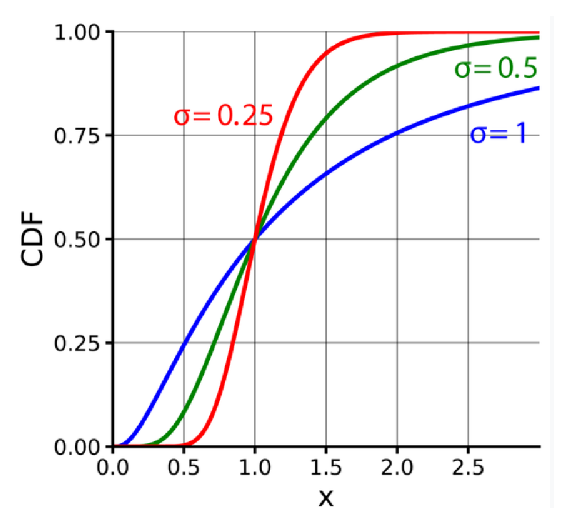
\includegraphics[width=0.25\paperwidth]{images/cdf_lognormal}
\par\end{centering}
\caption{Log Normal PDF (left) CDF (right)}
\end{figure}

\item \textbf{Multiple, Reciprocal, Power}
\begin{enumerate}
\item If $X\sim\mathcal{L}N(\mu,\sigma^{2})$, then $aX\sim\mathcal{L}N(\mu+\ln a,\sigma^{2})$
for $a>0$
\begin{enumerate}
\item If $X\sim\mathcal{L}N(\mu,\sigma^{2})$, then $\frac{1}{X}\sim\mathcal{L}N(-\mu,\sigma^{2})$
\item If $X\sim\mathcal{L}N(\mu,\sigma^{2})$, then If $X^{a}\sim\mathcal{L}N(a\mu,a^{2}\sigma^{2})$
\item If $X_{1},...,X_{n}\overset{i.i.d}{\sim}\mathcal{L}N(\mu_{i},\sigma_{i}^{2})$
then $Y=\mathop{\stackrel[i=1]{n}{\prod}X_{i}\sim}\mathcal{L}N(\mathop{\stackrel[i=1]{n}{\sum}}\mu_{i},\stackrel[i=1]{n}{\sum}\sigma_{i}^{2})$
\end{enumerate}
\end{enumerate}
\end{enumerate}
\begin{enumerate}[resume]
\item Population $\text{\ensuremath{X_{1}},...,\ensuremath{X_{n}\overset{i.i.d}{\sim}}}\mathcal{L}N(\mu,\sigma^{2})$
($\mu$ is unknown and $\sigma^{2}$ is unknown)
\begin{enumerate}[resume]
\item \textbf{Exponential family }form: $(x)^{-\frac{n}{2}}(2\pi\sigma^{2})^{-\frac{n}{2}}\exp\left(-n\frac{\mu^{2}}{2\sigma^{2}}\right)\exp\left(\frac{\mu}{\sigma^{2}}\sum_{i=1}^{n}\log x_{i}-\frac{1}{2\sigma^{2}}\sum_{i=1}^{n}\log x_{i}^{2}\right)$
\item The standard distribution is $\mathcal{L}N(0,1)$
\item \textbf{Minimal sufficient and complete statistic}: $\left(\sum_{i=1}^{n}\log X_{i},\sum_{i=1}^{n}\log X_{i}^{2}\right)$
\item \textbf{Fisher information}: $I=\text{diag}(\frac{1}{\sigma^{2}},\frac{2}{\sigma^{2}})$
\item \textbf{MLE} $\hat{\mu}={\displaystyle \frac{\sum_{i=1}^{n}\log X_{i}}{n}}$,
$\hat{\sigma}^{2}={\displaystyle \frac{\sum_{i=1}^{n}(\log X_{i}-\hat{\mu})^{2}}{n}}$
\end{enumerate}
\end{enumerate}
\pagebreak{}

\subsection{Weibull{*}}

In probability theory and statistics, the Weibull distribution is
a continuous probability distribution. It models a broad range of
random variables, largely in the nature of a time to failure or time
between events. Examples are maximum one-day rainfalls and the time
a user spends on a web page.
\begin{enumerate}
\item \textbf{PDF, CDF, MGF, mean and variance }of $X\sim\text{Weibull}(\lambda,k)$, 
\begin{enumerate}
\item \textbf{PDF}: 
\[
f(x)=\frac{k}{\lambda}\left(\frac{x}{\lambda}\right)^{k-1}e^{-(\frac{x}{\lambda})^{k}}
\]

\begin{center}
$x\geq0$, $\lambda>0$ is scale parameter, $k>0$ is shape parameter
\par\end{center}
\item \textbf{CDF}: $f(x)=(1-e^{-(\frac{x}{\lambda})^{k}})\cdot I_{[0,\infty)}(x)$
\item \textbf{MGF}: $M_{X}(t)=\mathop{\stackrel[n=0]{\infty}{\sum}\frac{t^{n}\lambda^{n}}{n!}\Gamma(1+\frac{n}{k})}$,
$k\geq1$
\item \textbf{Mean and Variance}: 
\[
E[X]=\lambda\Gamma(1+\frac{1}{k}),\,\,Var(X)=\lambda^{2}\left[\Gamma(1+\frac{2}{k})-\left(\Gamma(1+\frac{1}{k})\right)^{2}\right]
\]
\end{enumerate}
\begin{figure}[H]
\begin{centering}
\includegraphics[width=0.25\paperwidth]{images/dist_weibull} \includegraphics[width=0.25\paperwidth]{images/cdf_weibull}
\par\end{centering}
\caption{Weibull PDF (left) CDF (right)}
\end{figure}

\end{enumerate}
\begin{enumerate}[resume]
\item Random sample $X_{1},...,X_{n}\sim\text{Weibull}(\lambda,k)$ where
$\lambda$ is target parameter: exponential family? sufficient statistic?
minimal sufficient statistic? complete statistic? Fisher information?
UMVUE?

$k$ unknown

\textbf{Not exponential family }for $\lambda,k$ unknown

$\log f(x)=\log(\frac{k}{\lambda})+(k-1)\log(\frac{x}{\lambda})-(\frac{x}{\lambda})^{k}$

If $k$ known
\begin{enumerate}
\item \textbf{Exponential family }form: $f(x)=\frac{k}{\lambda^{k}}\left(x\right)^{k-1}e^{-(\frac{1}{\lambda}*x)^{k}}$
\item \textbf{Scale family}: The standard distribution is $\text{Exp}(1)$
and $\frac{X_{i}}{\beta}\sim\text{Exp}(1)$
\item \textbf{Minimal sufficient and complete statistic}: $\sum_{i=1}^{n}X_{i}^{k}$
\item \textbf{Fisher information}: $\frac{nk^{2}}{\lambda^{2}}$
\end{enumerate}
\item \textbf{Related Distributions}

\begin{figure}[H]
\begin{centering}
\includegraphics[width=0.4\paperwidth]{images/weibull}
\par\end{centering}
\caption{Weibull and related distributions}
\end{figure}

\begin{itemize}
\item If $X\sim\text{Weibull}(\lambda,\frac{1}{2})$ then $\sqrt{X}\sim\text{EXP}(\frac{1}{\sqrt{\lambda}})$
\end{itemize}
\end{enumerate}
\pagebreak{}

\subsection{Dirichlet{*}{*}}

In probability and statistics, the Dirichlet distribution (after Peter
Gustav Lejeune Dirichlet), often denoted $\text{Dir}(\boldsymbol{\alpha})$,
is a family of continuous multivariate probability distributions parameterized
by a vector $\boldsymbol{\alpha}$ of positive reals. It is a multivariate
generalization of the beta distribution, hence its alternative name
of multivariate beta distribution (MBD). Dirichlet distributions are
commonly used as prior distributions in Bayesian statistics, and in
fact, the Dirichlet distribution is the conjugate prior of the categorical
distribution and multinomial distribution.
\begin{enumerate}
\item \textbf{PDF, MGF, mean and variance} of $(X_{1},...,X_{K})\sim\text{Dir}(\alpha_{1},...,\alpha_{k}$) 
\begin{enumerate}
\item \textbf{PDF}: 
\[
\frac{1}{\text{B}(\boldsymbol{\alpha})}\stackrel[i=1]{K}{\prod}x_{i}^{\alpha_{i}-1}
\]

\begin{center}
$\mathop{\stackrel[i=1]{K}{\sum}x_{i}=1}$
\par\end{center}

\begin{center}
$\text{B}(\boldsymbol{\alpha})=\frac{\stackrel[i=1]{K}{\prod}\Gamma(\alpha_{i})}{\Gamma(\alpha_{0})}$
where $\alpha_{0}=\stackrel[i=1]{K}{\sum}\alpha_{i}$
\par\end{center}
\item \textbf{Mean and Variance}:
\end{enumerate}
\begin{center}
$E[X_{i}]=\frac{\alpha_{i}}{\alpha_{0}}$, $Var(X_{i})=\frac{\tilde{\alpha_{i}}(1-\tilde{\alpha_{i}})}{\alpha_{0}+1}$
where $\tilde{\alpha_{i}}=\frac{\alpha_{i}}{\alpha_{0}}$
\par\end{center}
\begin{enumerate}
\item \textbf{Covariance}: $\frac{-\alpha_{i}\alpha_{j}}{\alpha_{0}(\alpha_{0}+1)}$
for $i\neq j$
\end{enumerate}
\item \textbf{Conjugate prior }exists but not going to be useful here
\end{enumerate}
\begin{enumerate}[resume]
\item \textbf{Related Distributions}
\begin{enumerate}[resume]
\item For $K$ independent r.v.s $Y_{1}\sim\text{Gamma}(\alpha_{1},\beta)$,...,
$Y_{K}\sim\text{Gamma}(\alpha_{K},\beta)$, we have $V=\stackrel[i=1]{K}{\sum}Y_{i}\sim\text{Gamma}(\alpha_{0},\beta)$,
$X=\left(X_{1},...,X_{k}\right)=\left(\frac{Y_{1}}{V},...,\frac{Y_{K}}{V}\right)\sim\text{Dir}(\alpha_{1},...,\alpha_{K})$
\end{enumerate}
\item \textbf{Example problems} and key steps
\item Other notes
\begin{enumerate}[resume]
\item Multivariate generalization of Beta distribution
\end{enumerate}
\end{enumerate}
\pagebreak{}

\subsection{Inverse Gaussian{*}{*}{*}{*}{*}}

The inverse Gaussian distribution has several properties analogous
to a Gaussian distribution. The name can be misleading: it is an \textquotedbl inverse\textquotedbl{}
only in that, while the Gaussian describes a Brownian motion's level
at a fixed time, the inverse Gaussian describes the distribution of
the time a Brownian motion with positive drift takes to reach a fixed
positive level.

Its cumulant generating function (logarithm of the characteristic
function) is the inverse of the cumulant generating function of a
Gaussian random variable.
\begin{enumerate}
\item \textbf{PDF, MGF, mean and variance }of $X\sim\text{IG}(\mu,\lambda)$
\begin{enumerate}
\item \textbf{PDF}: 
\[
f(x)=\sqrt{\frac{\lambda}{2\pi x^{3}}}\exp\left[-\frac{\lambda(x-\mu)^{2}}{2\mu^{2}x}\right]
\]

\begin{center}
$0<x<\infty$
\par\end{center}

\begin{center}
$\mu>0$
\par\end{center}

\begin{center}
$\lambda>0$
\par\end{center}
\item \textbf{MGF}: $M_{X}(t)=\exp\left[\frac{\lambda}{\mu}\left(1-\sqrt{1-\frac{2\mu^{2}t}{\lambda}}\right)\right]$
\item \textbf{Mean and Variance}: 
\[
E[X]=\mu,\,\,Var(X)=\frac{\mu^{3}}{\lambda}
\]
\end{enumerate}
\begin{figure}[H]
\begin{centering}
\includegraphics[width=0.25\paperwidth]{images/dist_invgaussian}
\includegraphics[width=0.25\paperwidth]{images/cdf_invgaussian}
\par\end{centering}
\caption{Inverse Gaussian PDF (left) CDF (right)}
\end{figure}

\item \textbf{Sum and Scaling}
\begin{enumerate}
\item If $X_{i}\sim\text{IG}(\mu_{0}w_{i},\lambda_{0}w_{i}^{2})$ then $S=\stackrel[i=1]{n}{\sum}X_{i}\sim\text{IG}(\mu_{0}\stackrel[i=1]{n}{\sum}w_{i},\lambda_{0}(\stackrel[i=1]{n}{\sum}w_{i})^{2})$,
under condition that $\frac{\text{Var}(X_{i})}{\text{E}(X_{i})}=\frac{\mu_{0}^{2}w_{i}^{2}}{\lambda_{0}w_{i}^{2}}=\frac{\mu_{0}^{2}}{\lambda_{0}}$
is constant for all $i$
\item If $X\sim\text{IG}(\mu,\lambda)$, $tX\sim\text{IG}(t\mu,t\lambda)$
for $t>0$
\end{enumerate}
\end{enumerate}
\begin{enumerate}[resume]
\item Population $\text{\ensuremath{X_{1}},...,\ensuremath{X_{n}\overset{i.i.d}{\sim}}}\text{IG}(\mu,\lambda)$
\begin{enumerate}[resume]
\item \textbf{Exponential family }form: $f(x)=\exp\left[-\frac{\lambda}{2\mu^{2}}x+\frac{\lambda}{\mu}-\frac{\lambda}{2x}+\frac{1}{2}\log\lambda+\frac{1}{2}\log2\pi x^{3}\right]$
\item \textbf{Minimal sufficient and complete statistic}: $\left(\stackrel[i=1]{n}{\sum}X_{i},\stackrel[i=1]{n}{\sum}\frac{1}{X_{i}}\right)$
\item \textbf{Fisher information}: $I_{n}(\mu,\lambda)=\left(\frac{n\lambda}{\mu^{3}},\frac{n}{2\lambda^{2}}\right)$
\item \textbf{MLE} $\hat{\mu}=\bar{X}$, $\hat{\lambda}=\dfrac{n}{\stackrel[i=1]{n}{\sum}\left(\frac{1}{X_{i}}-\frac{1}{\bar{X}}\right)}$
\end{enumerate}
\item \textbf{Related Distributions}
\begin{enumerate}[resume]
\item \textbf{Pivot: }If $X\sim\text{IG}(\mu,\lambda)$, then $\dfrac{\lambda(X-\mu)^{2}}{\mu^{2}X}\sim\chi_{1}^{2}$
\item If $X_{i}\sim\text{IG}(\mu,\lambda)$ then $\stackrel[i=1]{n}{\sum}X_{i}\sim\text{IG}(n\mu,n^{2}\lambda)$
\item If $X_{i}\sim\text{IG}(\mu,\lambda)$ then $\bar{X}\sim\text{IG}(\mu,n\lambda)$
\item If $X_{i}\sim\text{IG}(\mu_{i},2\mu_{i}^{2})$ then $\stackrel[i=1]{n}{\sum}X_{i}\sim\text{IG}\left(\stackrel[i=1]{n}{\sum}\mu_{i},2\left(\stackrel[i=1]{n}{\sum}\mu_{i}\right)^{2}\right)$
\end{enumerate}
\end{enumerate}
\pagebreak{}

\subsection{Cauchy{*}}

Cauchy is the distribution of the ratio of two independent normally
distributed random variables with mean zero.

The Cauchy distribution is often used in statistics as the canonical
example of a \textquotedbl pathological\textquotedbl{} distribution
since both its expected value and its variance are undefined (but
see � Moments below). The Cauchy distribution does not have finite
moments of order greater than or equal to one; only fractional absolute
moments exist.{[}1{]} The Cauchy distribution has no moment generating
function.
\begin{enumerate}
\item \textbf{PDF, MGF, mean and variance }of $X\sim\text{Cauchy}(x_{0},\gamma)$;
$x_{0}$ location parameter, $\gamma$ scale parameter
\begin{enumerate}
\item \textbf{PDF}: 
\[
f(x)=\mathop{\frac{1}{\pi\gamma\left[1+\left(\frac{x-x_{0}}{\gamma}\right)^{2}\right]}}
\]

\begin{center}
$-\infty<x<\infty$
\par\end{center}

\begin{center}
$-\infty<x_{0}<\infty$
\par\end{center}

\begin{center}
$\gamma>0$
\par\end{center}
\item \textbf{CDF}: $F(x)=\frac{1}{\pi}\arctan\left(\frac{x-x_{0}}{\gamma}\right)+\frac{1}{2}$
\item \textbf{MGF}: Does not exist
\item \textbf{Mean and Variance}: 
\[
E[X]=\text{undefined},\,\,Var(X)=\text{undefined}
\]
\end{enumerate}
\begin{figure}[H]
\begin{centering}
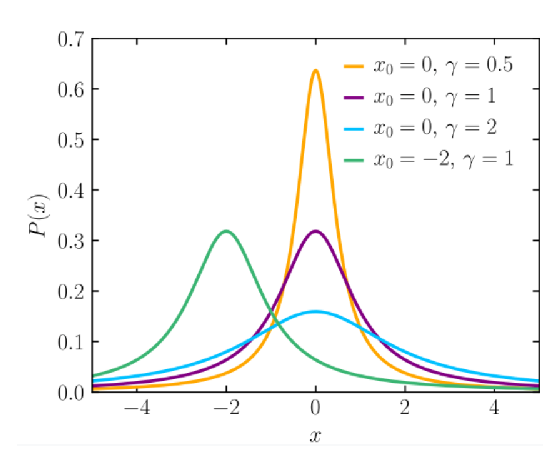
\includegraphics[width=0.25\paperwidth]{images/dist_cauchy} 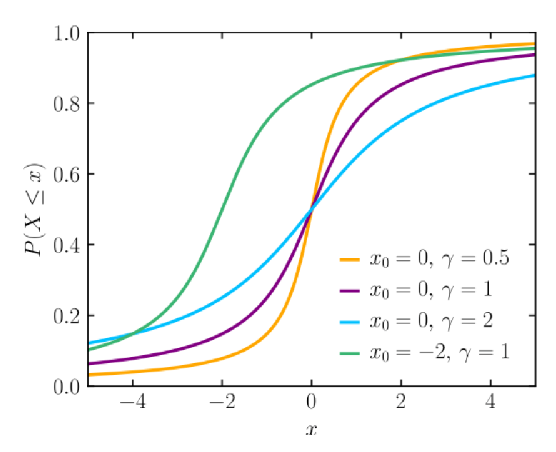
\includegraphics[width=0.25\paperwidth]{images/cdf_cauchy}
\par\end{centering}
\caption{Cauchy PDF (left) CDF (right)}
\end{figure}

\end{enumerate}
\begin{enumerate}[resume]
\item \textbf{Linearity} and \textbf{additivity}
\begin{enumerate}[resume]
\item If $X\sim\text{Cauchy}(x_{0},\gamma)$, then $kX+\ell\sim\text{Cauchy}(x_{0}k+\ell,\gamma|k|)$
\item If $X\sim\text{Cauchy}(x_{0},\gamma_{0})$ and $Y\sim\text{Cauchy}(x_{1},\gamma_{1})$
are independent, then $X+Y\sim\text{Cauchy}(x_{0}+x_{1},\gamma_{0}+\gamma_{1})$
and $X-Y\sim\text{Cauchy}(x_{0}-x_{1},\gamma_{0}+\gamma_{1})$
\item If $X\sim\text{Cauchy}(0,\gamma)$, then $\frac{1}{X}\sim\text{Cauchy}(0,\frac{1}{\gamma})$
\item If $X_{1},...,X_{n}\overset{i.i.d.}{\sim}\text{Cauchy}(0,1)$ standard
Cauchy distributed, then the sample mean $\frac{1}{n}\sum_{i=1}^{n}X_{i}=\bar{X}\sim\text{Cauchy}(0,1)$
is also standard Cauchy.
\end{enumerate}
\item Population $X_{1},...,X_{n}\sim\text{Cauchy}(x_{0},\gamma)$ ($\mu$
is unknown and $\sigma_{0}^{2}$ is known){*}{*}{*}{*}{*}
\item \textbf{Related Distributions}

\begin{figure}[H]
\begin{centering}
\includegraphics[width=0.35\paperwidth]{images/cauchy}
\par\end{centering}
\caption{Cauchy related distributions}
\end{figure}

\begin{enumerate}[resume]
\item If $X_{1}\sim N(0,1)$ and $X_{2}\sim N(0,1)$ are independent then
$\frac{X_{1}}{X_{2}}\sim\text{Cauchy}(0,1)$
\item $\text{Cauchy}(0,1)\sim t(\text{df}=1)$ Student's $t$ distribution
\item $\text{Cauchy}(\mu,\sigma)\sim t_{(\text{df}=1)}(\mu,\sigma)$ 
\item If $X\sim\text{Unif}(0,1)$ then $\tan(\pi(X-\frac{1}{2}))\sim\text{Cauchy}(0,1)$
\item If $X\sim\text{Cauchy}(x_{0},\gamma)$, then $\frac{1}{X}\sim\text{Cauchy}(\frac{x_{0}}{x_{0}^{2}+\gamma^{2}},\frac{\gamma}{x_{0}^{2}+\gamma^{2}})$
\end{enumerate}
\item \textbf{Example problems }and key steps
\end{enumerate}
\pagebreak{}

\subsection{Laplace (Double Exponential)}

In probability theory and statistics, the Laplace distribution is
a continuous probability distribution named after Pierre-Simon Laplace.
It is also sometimes called the double exponential distribution, because
it can be thought of as two exponential distributions (with an additional
location parameter) spliced together along the abscissa, although
the term is also sometimes used to refer to the Gumbel distribution.
The difference between two independent identically distributed exponential
random variables is governed by a Laplace distribution, as is a Brownian
motion evaluated at an exponentially distributed random time.
\begin{enumerate}
\item \textbf{PDF, CDF, MGF, mean and variance }of $X\sim\text{Laplace}(\mu,b)$;
$\mu$ is location parameter, $b$ is scale parameter. 
\begin{enumerate}
\item \textbf{PDF}: 
\[
f(x)=\frac{1}{2b}\exp\left(-\dfrac{|x-\mu|}{b}\right)
\]

\begin{center}
$-\infty<x<\infty$, $-\infty<\mu<\infty$ , $b>0$ 
\par\end{center}
\item \textbf{CDF}: $f(x)=$$\begin{cases}
\frac{1}{2}\exp\left(\dfrac{x-\mu}{b}\right) & x\leq\mu\\
1-\frac{1}{2}\exp\left(-\dfrac{x-\mu}{b}\right) & x>\mu
\end{cases}$
\item \textbf{MGF}: $M_{X}(t)=\frac{\mathop{\exp(\mu t)}}{1-b^{2}t^{2}}$,
$|t|<\frac{1}{b}$
\item \textbf{Mean and Variance}: 
\[
E[X]=\mu,\,\,Var(X)=2b^{2}
\]
\end{enumerate}
\begin{figure}[H]
\begin{centering}
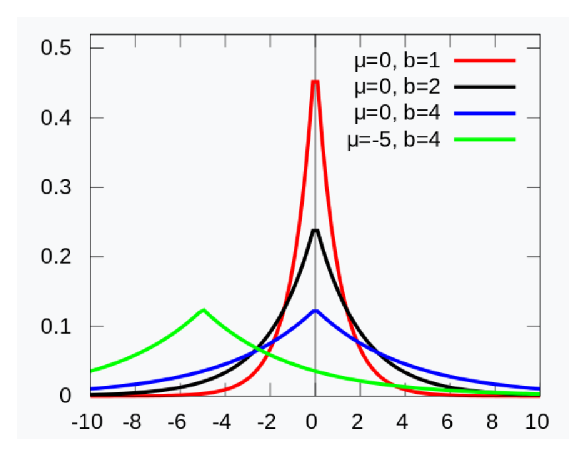
\includegraphics[width=0.25\paperwidth]{images/dist_laplace} 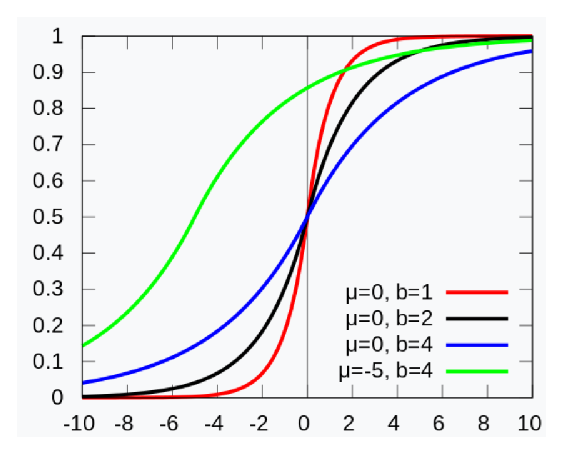
\includegraphics[width=0.25\paperwidth]{images/cdf_laplace}
\par\end{centering}
\caption{Laplace PDF (left) CDF (right)}
\end{figure}

\end{enumerate}
\begin{enumerate}[resume]
\item Random sample $X_{1},...,X_{n}\sim\text{Laplace}(\mu,b)$ where $\mu,b$
is target parameter: exponential family? sufficient statistic? minimal
sufficient statistic? complete statistic? Fisher information? UMVUE?
\begin{enumerate}
\item \textbf{Not exponential if $b$ or $\mu$ unknown. If $\mu$ known
exponential family }form: $f(x)=\frac{1}{2b}\exp\left(-\frac{1}{b}\stackrel[i=1]{n}{\sum}|x-\mu|\right)$
\item \textbf{Location-Scale family}: The standard distribution is $\text{Laplace}(0,1)$
and $\frac{X-\mu}{b}\sim\text{Laplace}(0,1)$
\item \textbf{Minimal sufficient and complete statistic}: $\sum_{i=1}^{n}|X_{i}-\mu|$
\item \textbf{Fisher information}: for $b=1$ $I_{n}(\mu)=n$, for $\mu=0$
$I_{n}(b)=\frac{n}{b^{2}}$
\end{enumerate}
\item \textbf{Related Distributions}

\begin{figure}[H]
\begin{centering}
\includegraphics[width=0.5\paperwidth]{images/laplace}
\par\end{centering}
\caption{Laplace and related distributions}
\end{figure}

\begin{itemize}
\item If $X\sim\text{Laplace}(\mu,b)$ then $kX+c\sim\text{Laplace}(k\mu+c,|k|b)$
\item If $X\sim\text{Laplace}(0,1)$ then $bX\sim\text{Laplace}(0,b)$
\item If $X\sim\text{Laplace}(0,b)$ then $|X|\sim\text{EXP}(b^{-1})$
\item If $X\sim\text{Laplace}(\mu,b)$ then $|X-\mu|\sim\text{EXP}(b^{-1})$
\item If $X,Y\sim\text{EXP}(\lambda)$, then $X-Y\sim\text{Laplace}(0,\lambda^{-1})$
\item If $X_{1},..,X_{4}\sim N(0,1)$ then $X_{1}X_{2}-X_{3}X_{4}\sim\text{Laplace}(0,1)$,
and $(X_{1}^{2}-X_{2}^{2}+X_{3}^{2}-X_{4}^{2})/2\sim\text{Laplace}(0,1)$
\item \textbf{Pivot: }If $X_{i}\sim\text{Laplace}(\mu,b)$ then $\frac{2}{b}\sum_{i=1}^{n}|X_{i}-\mu|\sim\chi_{2n}^{2}${*}
\item \textbf{Pivot: }If $X,Y\sim\text{Laplace}(\mu,b)$ then $\frac{|X-\mu|}{|Y-\mu|}\sim F_{2,2}$
\item If $X,Y\sim\text{Unif}(0,1)$ then $\log(\frac{X}{Y})\sim\text{Laplace}(0,1)$
\item If $X\sim\text{EXP}(\lambda)$ and $Y\sim\text{Bernoulli}(\frac{1}{2})$
are independent, then $X(2Y-1)\sim\text{Laplace}(0,\lambda^{-1})$
\item If $X\sim\text{EXP}(\lambda)$ and $Y\sim\text{EXP}(\nu)$ are independent,
then $\lambda X-\nu Y\sim\text{Laplace}(0,1)$
\end{itemize}
\end{enumerate}
\pagebreak{}

\subsection{$F$ Distribution}

In probability theory and statistics, the F-distribution or F-ratio,
also known as Snedecor's F distribution or the Fisher--Snedecor distribution
(after Ronald Fisher and George W. Snedecor), is a continuous probability
distribution that arises frequently as the null distribution of a
test statistic, most notably in the analysis of variance (ANOVA) and
other F-tests.
\begin{enumerate}
\item \textbf{PDF, CDF, MGF, mean and variance }of $X\sim F_{d_{1},d_{2}}$
\begin{enumerate}
\item \textbf{PDF}: 
\[
f(x)=\dfrac{\sqrt{\dfrac{(d_{1}x)^{d_{1}}d_{2}^{d_{2}}}{(d_{1}x+d_{2})^{d_{1}+d_{2}}}}}{x\text{B}\left(\frac{d_{1}}{2},\frac{d_{2}}{2}\right)}
\]

\begin{center}
$-\infty<x<\infty$
\par\end{center}
\item \textbf{CDF}: $f(x)=I_{\frac{d_{1}x}{d_{1}x+d_{2}}}\left(\frac{d_{1}}{2},\frac{d_{2}}{2}\right)$
\item \textbf{MGF}: DNE
\item \textbf{Mean and Variance}: 
\end{enumerate}
\begin{center}
$E[X]=\frac{d_{2}}{d_{2}-2}$ for $d_{2}>2$, $Var(X)=\frac{2d_{2}^{2}(d_{1}+d_{2}-2)}{d_{1}(d_{2}-2)^{2}(d_{2}-4)}$
for $d_{2}>4$
\par\end{center}

\begin{figure}[H]
\begin{centering}
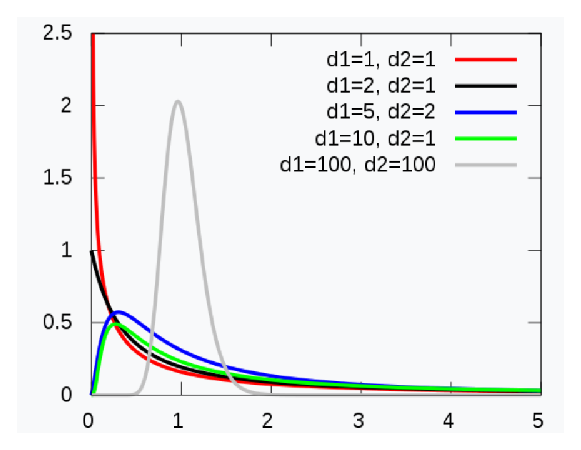
\includegraphics[width=0.25\paperwidth]{images/dist_F} 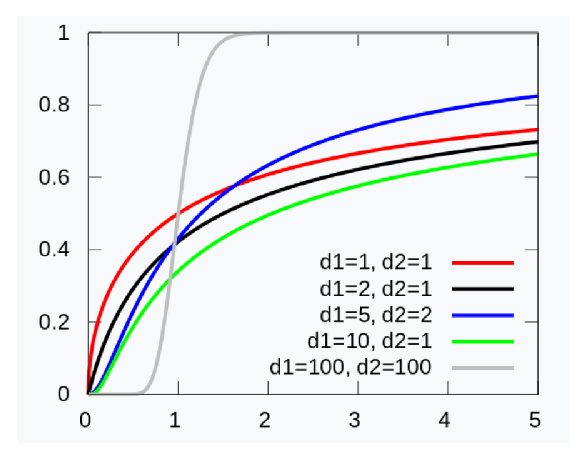
\includegraphics[width=0.25\paperwidth]{images/cdf_F}
\par\end{centering}
\caption{$F$ PDF (left) CDF (right)}
\end{figure}

\item \textbf{Related Distributions}

\begin{figure}[H]
\begin{centering}
\includegraphics[width=0.5\paperwidth]{images/f}
\par\end{centering}
\caption{$F$ and related distributions}
\end{figure}

\begin{itemize}
\item If $X\sim\chi_{d_{1}}^{2}$ and $Y\sim\chi_{d_{2}}^{2}$ are independent,
then $\dfrac{X/d_{1}}{Y/d_{2}}\sim F_{d_{1},d_{2}}$
\item If $X_{k}\sim\Gamma(\alpha_{k},\beta_{k})$ are independent, then
$\dfrac{\alpha_{2}\beta_{1}X_{1}}{\alpha_{1}\beta_{2}X_{2}}\sim F_{2\alpha_{1},2\alpha_{2}}$
\item If $X\sim\text{Beta}(\frac{d_{1}}{2},\frac{d_{2}}{2})$ then $\dfrac{d_{2}X}{d_{1}(1-X)}\sim F$ 
\begin{itemize}
\item Equivalently, if $X\sim F_{d_{1},d_{2}}$ then $\dfrac{d_{1}X/d_{2}}{1+d_{1}X/d_{2}}\sim\text{Beta}(\frac{d_{1}}{2},\frac{d_{2}}{2})$
\end{itemize}
\item If $X\sim F_{d_{1},d_{2}}$ then $Y=\underset{d_{2\rightarrow\infty}}{\lim}d_{1}X\sim\chi_{d1}^{2}$
\item If $X\sim F_{d_{1},d_{2}}$ then $X^{-1}\sim F_{d_{2},d_{1}}$
\item If $X\sim t_{n}$ then $X^{2}\sim F_{1,n}$, $X^{-2}\sim F_{n,1}$
\item If $X,Y\sim\text{Laplace}(\mu,b)$ then $\frac{|X-\mu|}{|Y-\mu|}\sim F_{2,2}$
\end{itemize}
\end{enumerate}
\pagebreak{}

\subsection{Student's $t$ Distribution}

In probability and statistics, Student's t-distribution (or simply
the t-distribution) $t_{\nu}$ is a continuous probability distribution
that generalizes the standard normal distribution. Like the latter,
it is symmetric around zero and bell-shaped.

However, $t_{\nu}$ has heavier tails and the amount of probability
mass in the tails is controlled by the parameter $\nu$ . For $\nu=1$
the Student's t distribution $t_{\nu}$ becomes the standard Cauchy
distribution, whereas for $\nu\rightarrow\infty$ it becomes the standard
normal distribution $\text{N}(0,1)$.

The Student's t-distribution plays a role in a number of widely used
statistical analyses, including Student's t-test for assessing the
statistical significance of the difference between two sample means,
the construction of confidence intervals for the difference between
two population means, and in linear regression analysis.
\begin{enumerate}
\item \textbf{PDF, CDF, MGF, mean and variance }of $X\sim t_{\nu}$
\begin{enumerate}
\item \textbf{PDF}: 
\[
f(x)=\dfrac{\Gamma\left(\frac{\nu+1}{2}\right)}{\sqrt{\nu\pi}\Gamma\left(\frac{\nu}{2}\right)}\left(1+\frac{x^{2}}{\nu}\right)^{-\frac{\nu+1}{2}}
\]

\begin{center}
$-\infty<x<\infty$
\par\end{center}
\item \textbf{MGF}: Undefined
\item \textbf{Mean and Variance}: 
\end{enumerate}
\begin{center}
$E[X]=0$ for $\nu>1$ otherwise undefined, $Var(X)=\frac{\nu}{\nu-2}$
for $\nu>2$, $\infty$ for $1<\nu\leq2$
\par\end{center}

\begin{figure}[H]
\begin{centering}
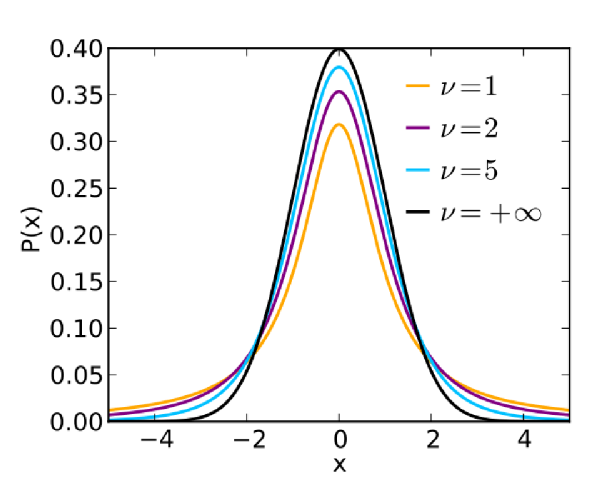
\includegraphics[width=0.25\paperwidth]{images/dist_t} 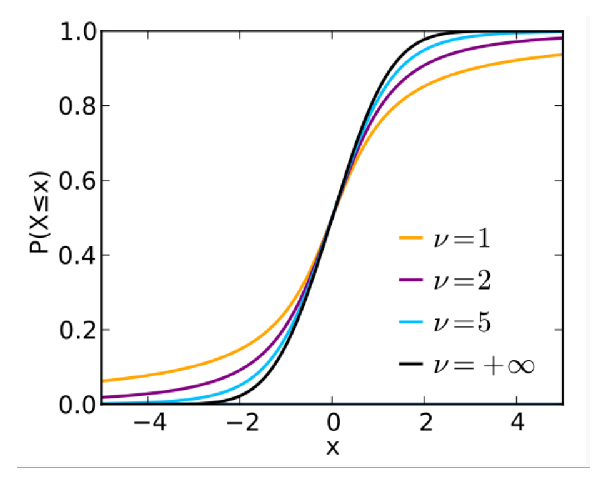
\includegraphics[width=0.25\paperwidth]{images/cdf_t}
\par\end{centering}
\caption{Student's $t$ PDF (left) CDF (right)}
\end{figure}

\item \textbf{Related Distributions}

\begin{figure}[H]
\begin{centering}
\includegraphics[width=0.5\paperwidth]{images/t}
\par\end{centering}
\caption{$t$ and related distributions}
\end{figure}

\begin{itemize}
\item \textbf{Pivot: }If $X_{1},...,X_{n}\overset{i.i.d.}{\sim}N(\mu,\sigma^{2})$
with sample mean $\bar{X}=\dfrac{\mathop{\stackrel[i=1]{n}{\sum}X_{i}}}{n}$
and sample variance $S^{2}=\frac{1}{n-1}\stackrel[i=1]{n}{\sum}(X_{i}-\bar{X})^{2}$
then $T=\frac{\bar{X}-\mu}{\sqrt{s^{2}/n}}\sim t_{n-1}$
\item \textbf{Pivot}: If $Z\sim N(0,1)$ and $U\sim\chi_{r}^{2}$ are independent,
then $T=\dfrac{Z}{\sqrt{U/r}}\sim t_{r}$
\end{itemize}
\end{enumerate}
\pagebreak{}

\subsection{$\chi_{n}^{2}$ Distribution}

Let us say that $X$ is distributed $\chi_{n}^{2}$. We know the following:
A $\chi_{n}^{2}$ is the sum of the squares of n independent standard
Normal r.v.s.
\begin{enumerate}
\item \textbf{PDF, CDF, MGF, mean and variance }of $X\sim t_{\nu}$
\begin{enumerate}
\item \textbf{PDF}: 
\[
f(x)=\dfrac{1}{2^{\frac{k}{2}}\Gamma\left(\frac{k}{2}\right)}x^{\frac{k}{2}-1}e^{-\frac{x}{2}}
\]

\begin{center}
$0\leq x<\infty$
\par\end{center}
\item \textbf{MGF}: $(1-2t)^{-\frac{k}{2}}$ for $t<\frac{1}{2}$
\item \textbf{Mean and Variance}:
\end{enumerate}
\begin{center}
$E[X]=k$, $Var(X)=2k$
\par\end{center}

\begin{figure}[H]
\begin{centering}
\includegraphics[width=0.25\paperwidth]{images/dist_chisq} \includegraphics[width=0.25\paperwidth]{images/cdf_chisq}
\par\end{centering}
\caption{$\chi_{n}^{2}$ PDF (left) CDF (right)}
\end{figure}

\item \textbf{Related Distributions}

\begin{figure}[H]
\begin{centering}
\includegraphics[width=0.5\paperwidth]{images/chisq}
\par\end{centering}
\caption{$\chi_{n}^{2}$ and related distributions}
\end{figure}

\begin{itemize}
\item If $Z_{1},...,Z_{n}\overset{i.i.d.}{\sim}N(0,1)$ then $Z_{i}^{2}\sim\chi_{1}^{2}$
and $Q=\stackrel[i=1]{n}{\sum}Z_{i}^{2}\sim\chi_{n}^{2}$
\item If $X\sim\chi_{k}^{2}$ then as $k\rightarrow\infty$, $\frac{(X-k)}{\sqrt{2k}}\overset{d}{\rightarrow}N(0,1)$
(CLT)
\item If $X\sim\text{Gamma}(\alpha,\beta)$, for $\alpha=\frac{n}{2}$,
$\beta=2$, $X\sim\chi_{n}^{2}$
\item If $X\sim\text{EXP (\ensuremath{\theta)}},$$\mathop{\stackrel[i=1]{n}{\sum}X_{i}}\sim\text{Gamma}(n,\theta)$
and $T=\frac{2\mathop{\stackrel[i=1]{n}{\sum}X_{i}}}{\theta}\sim\chi_{2n}^{2}$
\item If $X\sim F_{d_{1},d_{2}}$ then $Y=\underset{d_{2\rightarrow\infty}}{\lim}d_{1}X\sim\chi_{d1}^{2}$
\item If $X\sim\chi_{k}^{2}$ and $c>0$ then $cX\sim\text{Gamma}(\frac{k}{2},2c)$
\item If $X\sim\chi_{2}^{2}$ then $X\sim\text{EXP}(\frac{1}{2})$
\item If $X\sim\chi_{\nu_{1}}^{2}$ and $Y\sim\chi_{\nu_{2}}^{2}$ are independent,
then $\frac{X}{X+Y}\sim\text{Beta}(\frac{\nu_{1}}{2},\frac{\nu_{2}}{2})$
\item If $X\sim\text{Unif}(0.1)$ then $-2\log(X)\sim\chi_{2}^{2}$
\item If $X_{i}\sim\text{Laplace}(\mu,b)$ then $\frac{2}{b}\sum_{i=1}^{n}|X_{i}-\mu|\sim\chi_{2n}^{2}$
\end{itemize}
\end{enumerate}
\pagebreak{}

\subsection{Irwin-Hall}

A random variable with Irwin-Hall distribution is defined as the sum
of a number of independent random variables, each having a uniform
distribution. For this reason it is also known as the uniform sum
distribution. So, if $U_{i}\sim\text{Unif}(0,1)$ and $U_{1},...,U_{n}$
are $i.i.d.$ then $X=\stackrel[i=1]{n}{\sum}U_{i}\sim\text{IrwinHall}(n)$
\begin{enumerate}
\item \textbf{PDF, CDF, MGF, mean and variance} of $X\sim\text{IrwinHall}(n)$
\begin{enumerate}
\item \textbf{PDF}: 
\[
f(x)=\frac{1}{(n-1)!}\stackrel[k=1]{\lfloor x\rfloor}{\sum}(-1)^{k}{n \choose k}(x-k)_{+}^{n-1}
\]

\begin{center}
where $\left(x-k\right)_{+}=\begin{cases}
x-k & x-k\geq0\\
0 & x-k<0
\end{cases}$
\par\end{center}

\begin{center}
$0\leq x\leq n$
\par\end{center}

\begin{center}
$n\in\mathbb{N}$
\par\end{center}
\item \textbf{CDF}: $F(x)=\frac{1}{n!}\stackrel[k=1]{\lfloor x\rfloor}{\sum}(-1)^{k}{n \choose k}(x-k)_{+}^{n}$
\item \textbf{MGF}: $M_{X}(t)=\left(\frac{e^{t}-1}{t}\right)^{n}$
\item \textbf{Mean and Variance}: 
\[
E[X]=\frac{n}{2},\,\,Var(X)=\frac{n}{12}
\]
\end{enumerate}
\end{enumerate}
\begin{enumerate}[resume]
\item \textbf{Example problems }and key steps
\end{enumerate}

\end{document}
